%-----------------------------------------------
%  Engineer's & Master's Thesis Template
%  Copyleft by Artur M. Brodzki & Piotr Woźniak
%  Warsaw University of Technology, 2019-2022
%-----------------------------------------------

\documentclass[
    bindingoffset=5mm,  % Binding offset
    footnoteindent=3mm, % Footnote indent
    hyphenation=true    % Hyphenation turn on/off
]{src/wut-thesis}

% ---- ---- ---- ----
% Packages
% ---- ---- ---- ----
\usepackage{tikz}
\usepackage{float}
\usepackage{longtable}
\usepackage{tabularx}
\usepackage{xltabular}
\usepackage{booktabs}
\usepackage{tabularray}

% ---- ---- ---- ----
% Packages Configuration
% ---- ---- ---- ----
\usetikzlibrary{shapes.geometric, arrows.meta, positioning}
\DefTblrTemplate{caption-tag}{default}{\small \textbf{Tabela\hspace{0.25em}\thetable}}
\DefTblrTemplate{caption-sep}{default}{.\enskip}
\DefTblrTemplate{caption-text}{default}{\small \InsertTblrText{caption}}
\DefTblrTemplate{contfoot-text}{default}{Kontynuacja na następnej stronie.}
\DefTblrTemplate{conthead-text }{default}{}

\newcolumntype{R}{>{\raggedleft\arraybackslash}X}

% ---- ---- ---- ----
% Writing utilities
% ---- ---- ---- ----
\newcommand{\todo}[1]{%
    \definecolor{Red}{HTML}{ff6b6b}
    \tikzstyle{box} = [rectangle, minimum width=15cm, minimum height=1cm, line width=2pt, text centered, draw=Red, align=left, inner sep=10pt, Red]

    \begin{tikzpicture}
        \node [box] { 
            \textbf{Ta sekcja wymaga rozwinięcia}\\%
            \parbox{\dimexpr\linewidth-2em}{#1}%
        };
    \end{tikzpicture} 
}
\newcommand{\question}[1]{%
    \definecolor{Blue}{HTML}{54a0ff}
    \tikzstyle{box} = [rectangle, minimum width=15cm, minimum height=1cm, line width=2pt, text centered, draw=Red, align=left, inner sep=10pt, Blue]

    \begin{tikzpicture}
        \node [box] { 
            \textbf{Pytanie}\\%
            \parbox{\dimexpr\linewidth-2em}{#1}%
        };
    \end{tikzpicture} 
}

% ---- ---- ---- ----
% Title page
% ---- ---- ---- ----
\graphicspath{{tex/imagesg/}}
\addbibresource{bibliography.bib}

% ---- ---- ---- ----
% Thesis template configuration
% ---- ---- ---- ----
\facultyeiti{}
\EngineerThesis{} 
\langpol{}

\begin{document}

% ---- ---- ---- ----
% Title page
% ---- ---- ---- ----
\instytut{Informatyki}
\kierunek{Informatyka}
\specjalnosc{Sztuczna Inteligencja}
\title{
    Projekt aplikacji do monitorowania DNA w środowisku
}

% English title
\engtitle{
    Design of an application for monitoring DNA in the environment
}

% Polish title
\poltitle{
    Projekt aplikacji do monitorowania DNA w środowisku
}

\author{Patryk Filip Gryz}
\album{318657}
\promotor{dr hab.\ inż. Robert Nowak}
\date{\the\year}
\maketitle

% ---- ---- ---- ----
% Abstract in polish
% ---- ---- ---- ----
\cleardoublepage{}

\abstract{}

Test

\keywords{}

Słowo kluczowe 1, słowo kluczowe 2, słowo kluczowe 3.



% ---- ---- ---- ----
% Abstract in english
% ---- ---- ---- ----
\cleardoublepage{}

\secondabstract{}
The aim of this thesis is to develop an application for analyzing genetic material DNA from various organisms collected from the environment. The application uses a database of genetic sequences and introduced an improvement in the analysis process by using various methods, including machine learning.
Taxonomic classification of genetic sequences was used to perform genetic material analysis. Optimization of the process was achieved by clustering genetic sequences and selecting representatives of the sequences that were used for taxonomic classification. The thesis implemented two classical methods: one using sequence alignments and the other based on $k$-mers. An original method was also developed, based on machine learning, using artificial neural networks with contrastive learning. A console application was created to conduct the analysis process, and a web application was developed to allow users to submit genetic material analysis requests. The implementation was done in the Rust programming language.
Qualitative experiments were conducted, comparing the implemented methods against a full taxonomic classification of all sequences, as well as performance experiments, evaluating the execution time of the entire process. The results showed that the custom method demonstrated the highest classification quality and the fastest execution time compared to the other metods.


\secondkeywords{}
DNA sequences, taxonomic classification,  metagenomics, artificial neural networks, contrastive learning

\pagestyle{plain}

% ---- ---- ---- ----
% Table of contents
% ---- ---- ---- ----
\cleardoublepage{}
\tableofcontents

% ---- ---- ---- ----
% Chapters
% ---- ---- ---- ----
\cleardoublepage{}
\pagestyle{headings}

\clearpage
\section{Wprowadzenie}
    Bibliografia \cite{knuth1984texbook}.

\clearpage
\section{Wstęp teoretyczny}

    % ===== ===== ===== =====
    % PRZEGLĄD LITERATURY
    % ===== ===== ===== ===== 
    \subsection{Przegląd literatury}

        \todo{
            \begin{enumerate}
                \item {podsumowanie dotychczasowych badań, publikacji i prac naukowych,}
                \item {krótkie przedstawienie osiągnięć w analizowanych obszarze,}
                \item {wskazanie luki badawczej}
            \end{enumerate}
        }

    % ===== ===== ===== =====
    % KLUCZOWE POJĘCIA I DEFINICJE
    % ===== ===== ===== ===== 
    \subsection{Kluczowe pojęcia i definicje}

        \subsubsection{Sekwencja DNA}

            Sekwencja DNA to sekwencja genetyczna stanowiąca zapis informacji genetycznej, który w sposób symboliczny odwzorowuje strukturę cząstki DNA, stosując alfabet złożony z czterech symboli: \texttt{A, T, C, G}. Każdy z symboli odnosi się do jednej z zasad azotowych zawartych w nukleotydach tworzących cząsteczkę DNA, odpowiednio: adeniny, tyminy, cytozyny oraz guaniny.

        \subsubsection{$k$-mer}

            $k$-mer to podsłowo sekwencji genetycznej o długości $k$. Dla danego alfabetu $G$ składające się z $n$ symboli istnieje dokładnie $n^k$ różnych $k$-merów o długości $k$. Sekwencja genetyczna o długości $m$ zawiera dokładnie $m - k + 1$ $k$-merów o długości $k$.


        \subsubsection{Dopasowanie sekwencji}

            Proces dopasowania sekwencji polega na wyrównaniu ich symboli w celu maksymalizacji ich wzajemnego podobieństwa, co realizowane może być poprzez wstawianie przerw (ang. \textit{gaps}) między symbolami sekwencji wejściowych. Dopasowanie sekwencji może być realizowane na dwa sposoby: lokalnie, gdzie maksymalizowane jest podobieństwo fragmentów sekwencji niezależnie od ich położenia oraz globalnie, gdzie maksymalizowane jest podobieństwo całych sekwencji. Wynikiem dopasowania są sekwencje z opcjonalnie wstawionymi przerwami oraz miara jakości dopasowania lub miara podobieństwa między sekwencjami.

        \subsubsection{Uczenie kontrastowe}
            
            Uczenie kontrastowe (ang. \textit{contrastive learning})\cite{Bromley1993} jest metodą uczenia maszynowego polegającą na maksymalizacji podobieństwa między podobnymi próbkami oraz minimalizacji podobieństwa między niepodobnymi próbkami. Wykorzystuje ona miary niepodobieństwa między reprezentacjami do nauki odróżniania kluczowych cech próbek. Zastosowanie tej metody pozwala na redukcję wymiarowości danych przy jednoczesnym zachowaniu właściwości podobieństwa i niepodobieństwa między danymi wejściowymi.

        \subsubsection{Podobieństwo kosinusowe}

            Podobieństwo kosinusowe to miara, która określa jak bardzo zbliżone, są wektory pod względem kierunku w przestrzeni wielowymiarowej. Miara wyrażona jest za pomocą kosinusa kąta między wektorami i przyjmuje wartości z zakresu $[-1; 1]$, gdzie $1$ określa pełne podobieństwo, a $-1$ całkowity brak podobieństwa. Podobieństwo kosinusowe wyrażone jest wzorem:

            \begin{equation}
                similarity_{cosine}(A, B) = \cos{\theta} = \frac{A \cdot B}{\|A\| \|B\|} = \frac{
                    \sum^{n}_{i = 1}A_i B_i
                }{
                    \sqrt{
                        \sum^{n}_{i = 1}A_i^2
                    }
                    \cdot
                    \sqrt{
                        \sum^{n}_{i = 1}B_i^2
                    }
                }
            \end{equation}

            gdzie,
            \begin{align*}
                A, B -& \text{porównywane wektory,} \\
                \theta -& \text{kąt między wektorami $A$ i $B$,} \\
                A_j, B_j -& \text{$j$-ty element wektora odpowiednio $A$ oraz $B$.}
            \end{align*}

        \subsubsection{Niepodobieństwo kosinusowe}

            Niepodobieństwo kosinusowe to miara, która określa jak bardzo wektory różnią się pod względem kierunku. Wyrażone jest wzorem:

            \begin{equation}
                dissimilarity_{cosine}(A, B) = 1 - similarity_{cosine}(A, B)
                \label{Equation:CosineDissimilarity}
            \end{equation}

            gdzie,
            \begin{align*}
                A, B -& \text{porównywane wektory,} \\
                similarity_{cosine}(A, B) -& \text{podobieństwo kosinusowe między wektorami $A$ i $B$.}
            \end{align*}

        \subsubsection{Format FASTA}

            Format FASTA jest to tekstowy format zapisu sekwencji nukleotydów. Nukleotydy reprezentowane są przez znaki \texttt{A, C, T, G}. Format składa się z jednej linii rozpoczynającej się znakiem \texttt{>} zawierającej identyfikator i opcjonalny opis oraz kolejnych linii zawierających sekwencję nukleotydów. Możliwy jest zapis wielu sekwencji w formacie FASTA w jednym pliku poprzez połączenie wielu sekwencji zapisanych w tym formacie.

        \subsubsection{Format FASTQ} 

            Format FASTQ jest to tekstowy format zapisu sekwencji nukleotydów, który zawiera dodatkowo informacje o jakości sekwencjonowania. Format umożliwia zapis wielu sekwencji w jednym pliku. Zapis każdej sekwencji składa się z czterech części: 
            \begin{enumerate}
                \item {
                    Pierwsza część to linia rozpoczynająca się od znaku \texttt{@} i zawierająca identyfikator oraz opcjonalny opis sekwencji.
                }
                \item {
                    Druga część to linie zawierające sekwencję nukleotydów, reprezentowanych przez znaki \texttt{A, C, T, G}.
                }
                \item {
                    Trzecia część to znak \texttt{+}, który oddziela sekwencję od informacji o jakości.
                }
                \item {
                    Czwarta część to linie zawierające zapis informacji o jakości sekwencjonowania. Informacja ta jest zakodowana za pomocą pojedynczych znaków ASCII, które odpowiadają jakości poszczególnych nukleotydów w sekwencji.
                }
            \end{enumerate}

        \subsubsection{\texttt{BLASTn}}

            \texttt{BLASTn} (ang. \textit{Basic Local Alignment Search Tool for Nucleotides}) to wariant narzędzia bioinformatycznego \texttt{BLAST}, zaprojektowany do porównywania sekwencji nukleotydów. Umożliwia wyszukiwanie podobieństw między analizowanymi sekwencjami nukleotydów a sekwencjami znajdującymi się w wybranej bazie sekwencji nukleotydów. Może być wykorzystywany do przeprowadzania klasyfikacji taksonomicznej.

        \todo {
            Algorytm k-medoidów
        }

        \todo {
            Klasyfikacja taksonomiczna
        }

    % ===== ===== ===== =====
    % METODY I PODEJŚCIA
    % ===== ===== ===== ===== 
    \subsection{Metody i podejścia}

        \todo{
            \begin{enumerate}
                \item {Przedstawienie najpopularniejszych metod, podejść lub algorytmów wykorzystywanych w literaturze przedmiotu w kontekście tematu pracy.,}
                \item {Opis sposobów, w jaki te metody zostały zaadoptowane lub zmodyfikowane w pracy.}
                \item {Wskazanie zalet i wad poszczególnych metod.}
            \end{enumerate}
        }

        \todo {
            Kraken2 itd.
        }

        \todo {
            Needleman-Wunsch
        
            Wady: wolne określanie podobieństwa 
            Zalety: uwzględnia strukturę
        }   

        \todo {
            KMer

            Wady: nie uwzględnia struktury
            Zalety: szybkie, łatwe w wykorzystaniu, SOTA
        }

    % ===== ===== ===== =====
    % TEORETYCZNE PODSTAWY PROBLEMU
    % ===== ===== ===== ===== 
    \subsection{Teoretyczne podstawy problemu}

        \todo{
            \begin{enumerate}
                \item {Szczegółowe przedstawienie teoretycznych podstaw, które stanowią tło dla rozwiązania danego problemu w pracy,}
                \item {Omówienie teorii, które są bezpośrednio związane z problemem badawczym (np. modele matematyczne, algorytmy, teorie z dziedziny nauk komputerowych, inżynierii, matematyki).}
            \end{enumerate}
        }
            
%         \subsubsection{Algorytm Needlema-Wunscha}
        
%            Algorytm Needlemana-Wunscha stanowi metodę wykorzystywaną do ustalania globalnego dopasowania pomiędzy dwiema sekwencjami \cite{NeedlemanWunsch1970}. Metoda ta polega na skonstruowaniu macierzy podobieństwa pomiędzy sekwencjami zgodnie z ustalonymi regułami:

%            \begin{equation}
%                 \begin{aligned}
%                     D_{i,0} &= i \cdot g, & \text{dla } & i \in [0, n] \\
%                     D_{0,j} &= j \cdot g, & \text{dla } & j \in [1, m] \\
%                     D_{i,j} &= \max
%                     \begin{cases}
%                     D_{i - 1, j} + g \\
%                     D_{i, j - 1} + g \\
%                     D_{i - 1, j - 1} + s(A_i, B_j)
%                     \end{cases}, & \text{dla } & i \in (0, n] \text{ oraz } j \in (0, m]
%                 \end{aligned}
%                 \label{Equation:NeedlemanWunsch}
%             \end{equation}

%             gdzie,
%             \begin{align*} 
%                 & g, s(A_i, B_j) \in \mathbb{R} \\
%                 A, B -& \text{porównywane sekwencje}, \\
%                 n, m -& \text{długości sekwencji } A \text{ oraz } B, \\
%                 D -& \text{macierz podobieństwa o rozmiarach } n \text{ x } m, \\
%                 g -& \text{kara za przerwę}, \\
%                 s(A_i, B_j) -& \text{podobieństwo między  } i\text{-tym elementem w sekwencji A,} \\ 
%                 & \text{a } j \text{-tym elementem w sekwencji B}. \\
%             \end{align*}

%             Wartość znajdująca się w $D_{n, m}$ określa liczbowo jakość globalnego dopasowania sekwencji.


\clearpage
\section{Analiza literatury}

**TODO** [ok. 15 stron]

\begin{enumerate}
    \item Opis problemu
    \item Opis rozwiązań problemu
    \item Opis algorytmów rozwiązujących problem
    \item Opis narzędzi (tutaj: Rust, Python itd.) + używane biblioteki
\end{enumerate}

% chktex-file 44
\clearpage
\section{Projekt i Implementacja}

    % ===== ===== ===== =====
    % WYMAGANIA FUNKCJONALNE I NIEFUNKCJONALNE
    % ===== ===== ===== ===== 
    \subsection{Wymagania funkcjonalne i niefunkcjonalne}

        \subsubsection{Wymagania funkcjonalne}

            \begin{itemize}
                \item Aplikacja powinna umożliwiać przeprowadzanie klasyfikacji taksonomicznej dla wprowadzonych sekwencji.
                \item Aplikacja powinna umożliwiać wybór metody grupowania sekwencji genetycznych.
                \item Aplikacja powinna zawierać zaimplementowane trzy metody grupowania sekwencji genetycznych.
                \item Aplikacja powinna umożliwiać porównanie jakości klasyfikacji taksonomicznej wykonanej przy użyciu różnych metod grupowania.
                \item Aplikacja powinna umożliwiać zapis wyników w formacie JSON.
            \end{itemize}

        \subsubsection{Wymagania niefunkcjonalne}

            \begin{itemize}
                \item Aplikacja powinna być wykonana przy wykorzystaniu kompilowanego wysoko wydajnego języka programowania.
                \item Implementacja powinna zawierać testy jednostkowe poszczególnych modułów i funkcji.
            \end{itemize}

    % ===== ===== ===== =====
    % MODEL ARCHITEKTURY C4
    % ===== ===== ===== =====
    \subsection{Model architektury rozwiązania}

        Architektura rozwiązania została przedstawiona w postaci modelu C4\cite{C4}. Model ten opisuje architekturę na czterech poziomach: kontekstowym (ang. \textit{System context}), kontenerów (ang. \textit{Container}), komponentów (ang. \textit{Component}) oraz kodu, przechodząc od najbardziej abstrakcyjnego spojrzenia na architekturę rozwiązania do kodu implementacji. Na rysunku~\ref{Picture:App:C4:Context} przedstawiono diagram kontekstowy modelu architektury, przedstawia on relacje między użytkownikami systemu a systemem oraz relacje między systemem a systemami zewnętrznymi. Na rysunku~\ref{Picture:App:C4:Container} przedstawiono natomiast diagram kontenerów modelu architektury, który przedstawia relacje między użytkownikami a poszczególnymi aplikacjami, biblioteką oraz systemami zewnętrznymi.

        \begin{figure}
            \begin{center}
                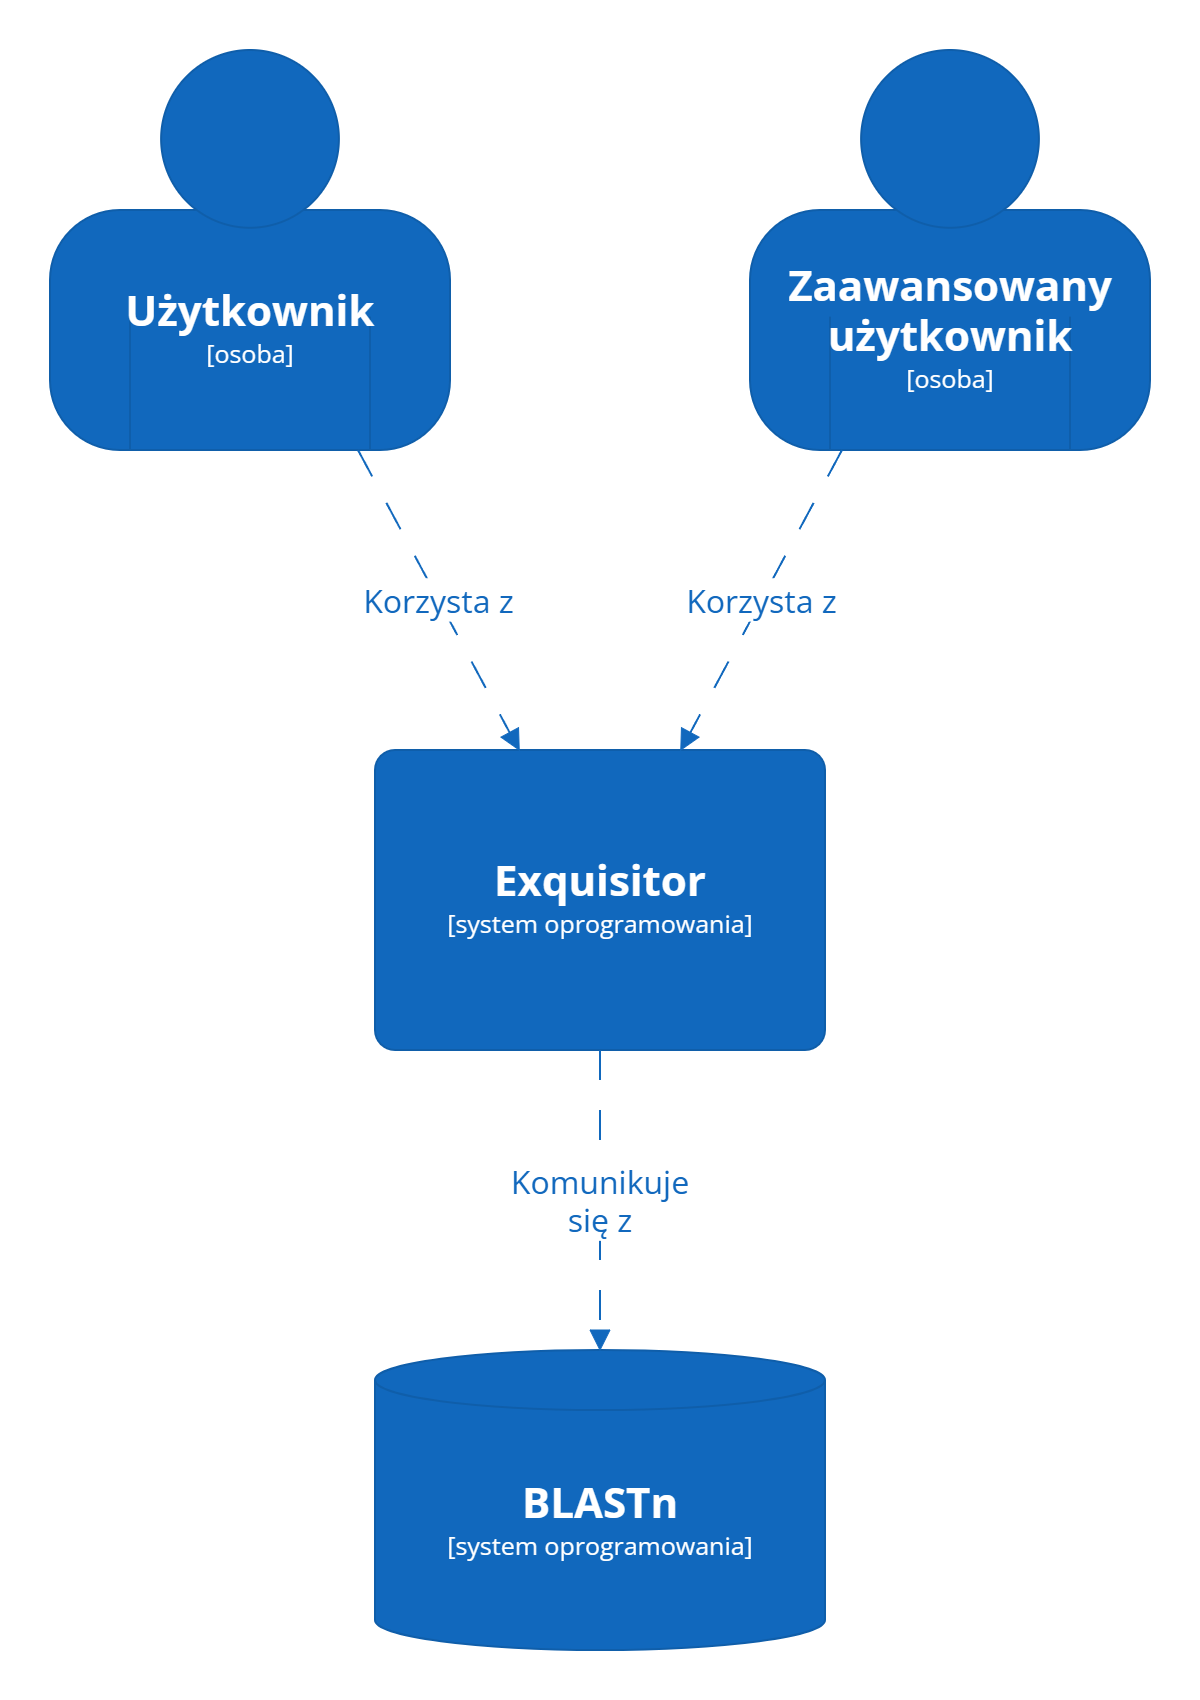
\includegraphics[width=\textwidth]{tex/pictures/app/c4_system_context.png}
            \end{center}
            \caption{
                Diagram kontekstowy modelu architektury.
            }\label{Picture:App:C4:Context}
        \end{figure}

        \begin{figure}
            \begin{center}
                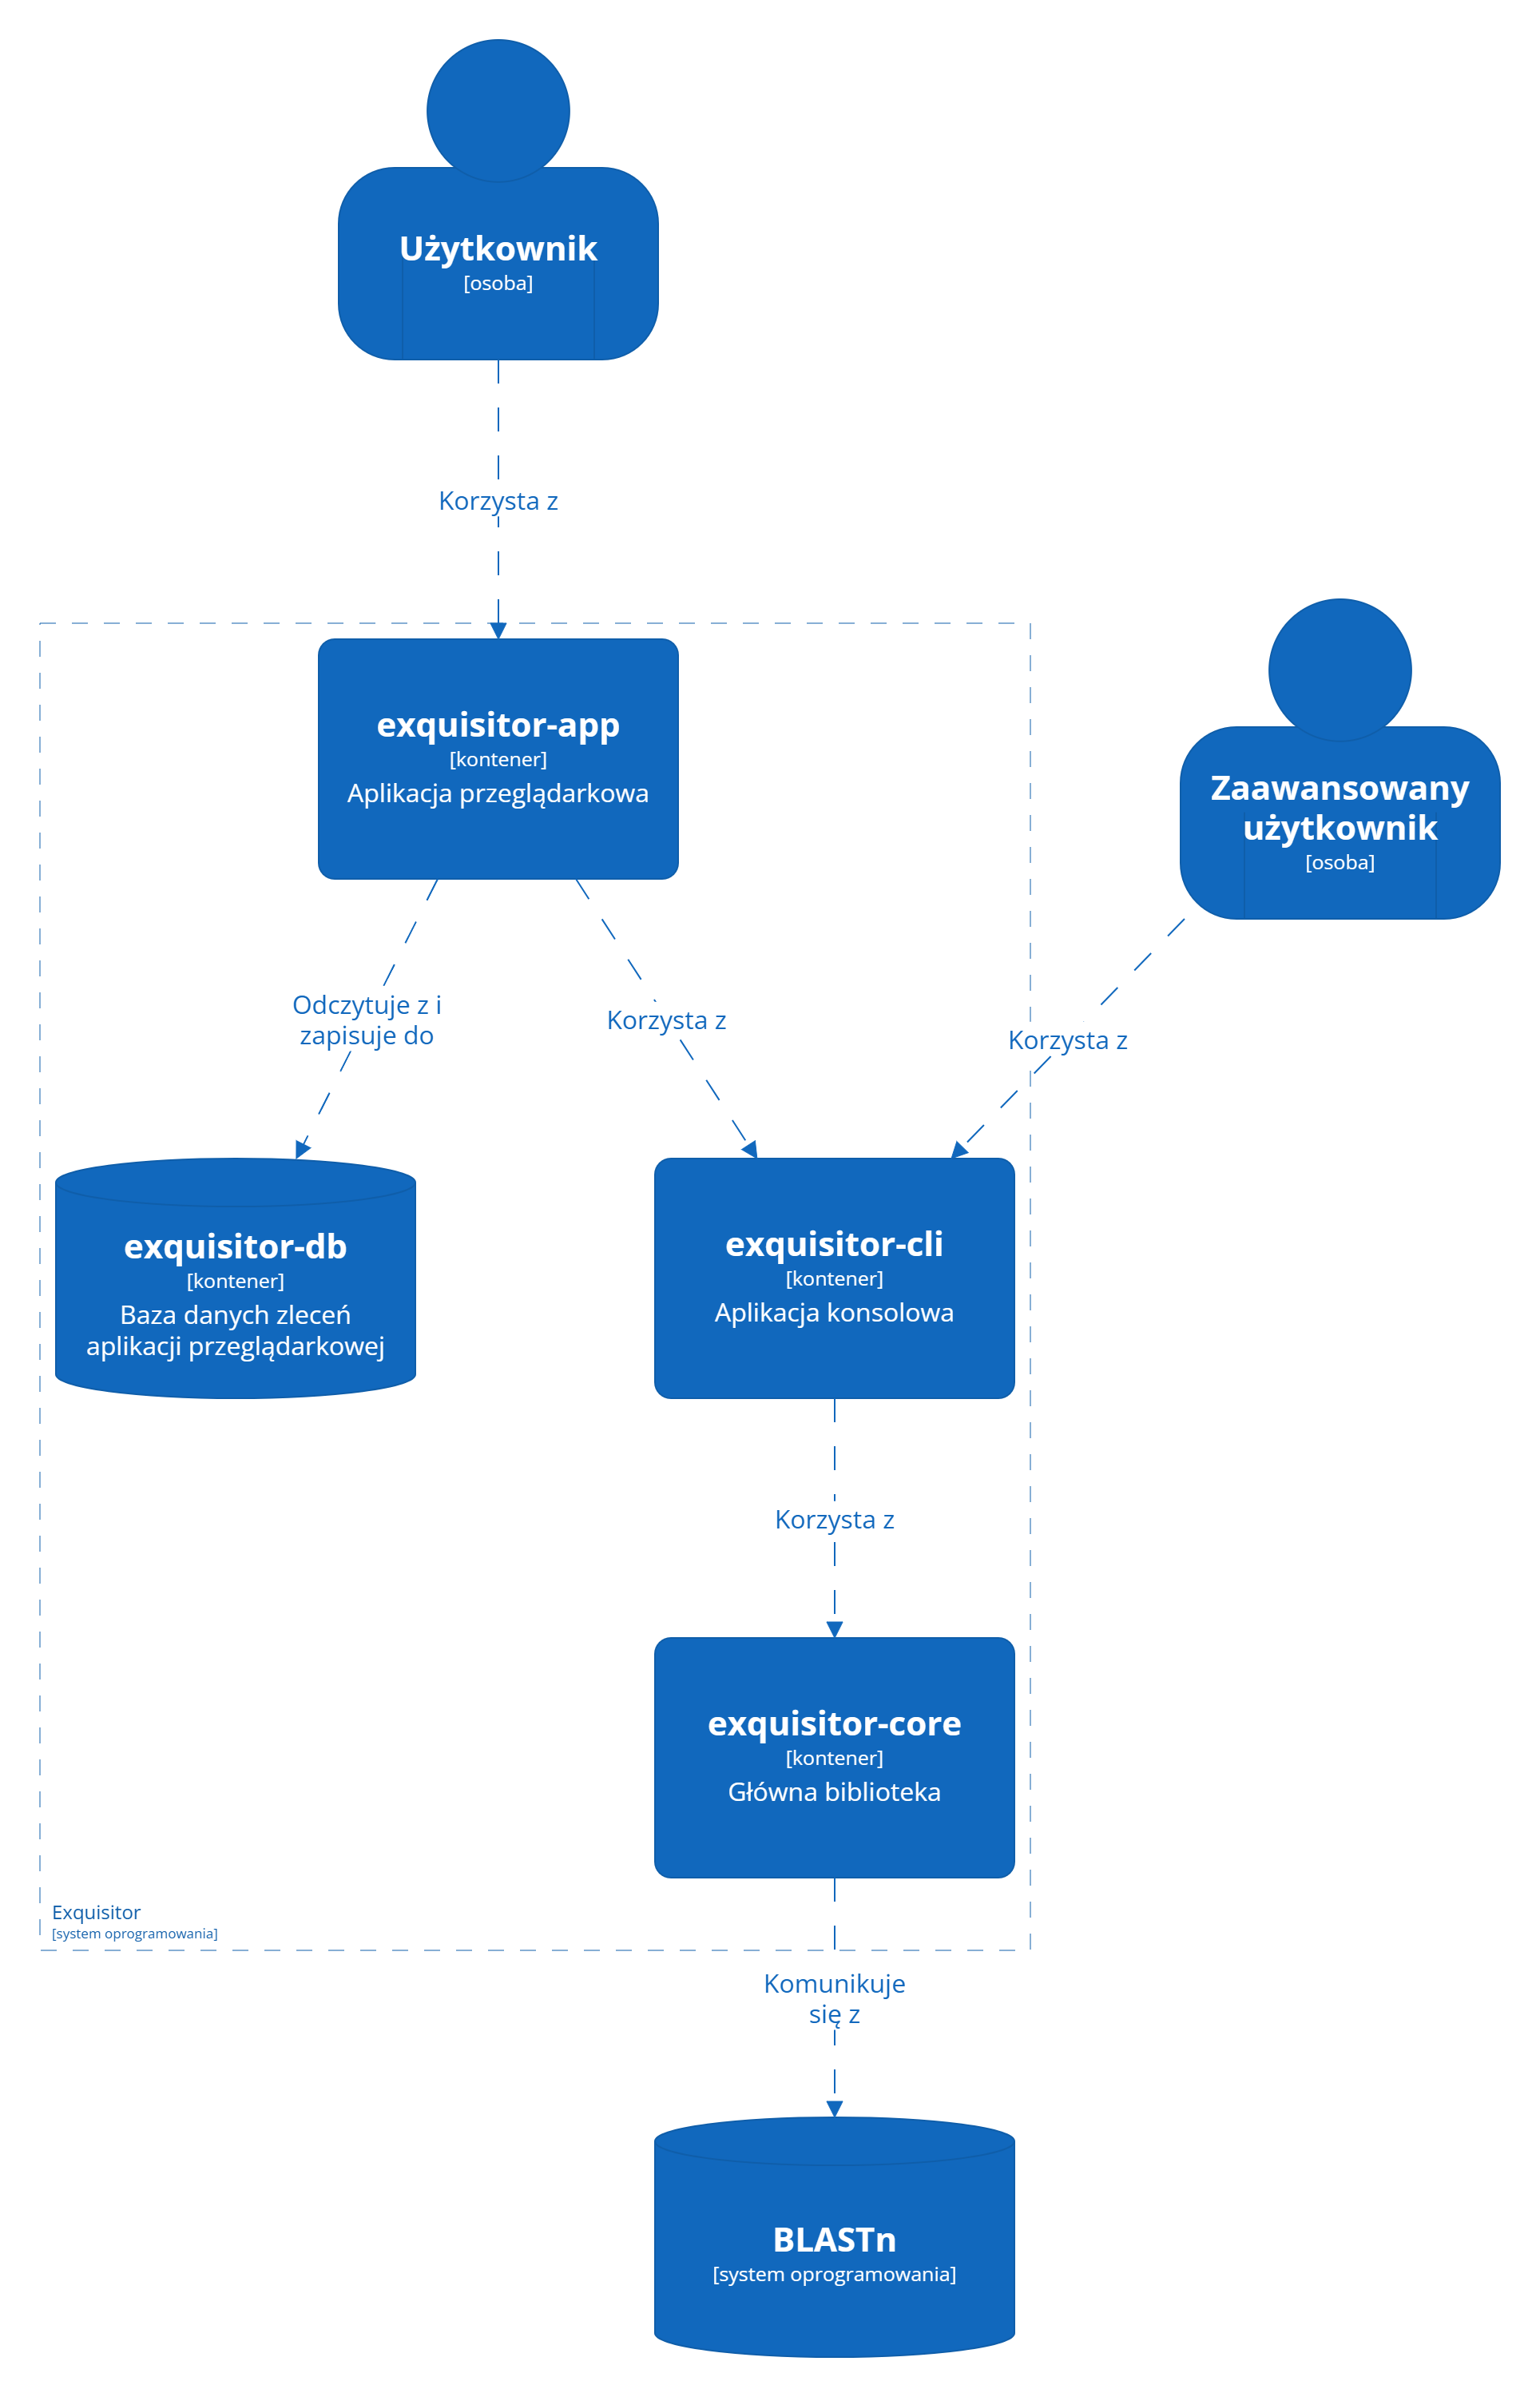
\includegraphics[width=\textwidth]{tex/pictures/app/c4_container.png}
            \end{center}
            \caption{
                Diagram komponentów modelu architektury.
            }\label{Picture:App:C4:Container}
        \end{figure}

    % ===== ===== ===== =====
    % OPIS ROZWIĄZANIA
    % ===== ===== ===== ===== 
    \subsection{Opis rozwiązania}

        Centralnym elementem rozwiązania jest potok przetwarzania, zaprojektowany z myślą o elastycznej konfiguracji oraz możliwości zastosowania różnych metod grupowania sekwencji DNA. Elementy potoku zostały zaimplementowane w bibliotece \textit{exquisitor-core}, w postaci funkcji oraz rekordów. Realizacja potoku została umieszczona w aplikacji konsolowej, która wykorzystuje tę bibliotekę. Aplikacja umożliwia uruchamianie i konfigurację potoku, oferując dostęp do dostępnych metod. Zawiera również polecenia pomocnicze, które zostały przygotowane w celu przeprowadzenia eksperymentów.

        Dodatkowo stworzono aplikację przeglądarkową, oferującą prosty interfejs w postaci strony internetowej. Umożliwia ona użytkownikowi zlecanie klasyfikacji taksonomicznej dla przesłanych sekwencji DNA.\@Do realizacji zleconych zadań aplikacja przeglądarkowa korzysta z aplikacji konsolowej.

        Ostatnim komponentem rozwiązania jest sieć neuronowa, której elementy zostały zawarte w bibliotece \textit{exquisitor-core}. 

        Biblioteka, aplikacja konsolowa oraz aplikacja przeglądarkowa zostały umieszczone w oddzielnych skrzynkach (ang. \textit{crate}) w ramach jednego rozwiązania. Dzięki temu możliwe jest rozdzielenie odpowiedzialności między poszczególnymi elementami, niezależny rozwój kodu oraz umożliwienie wykorzystania biblioteki w innych aplikacjach.

        % ----- ----- ----- ----- 
        % OPIS POTOKU
        % ----- ----- ----- -----

        \subsubsection{Potok przetwarzania}

            Potok przetwarzania składa się z szeregu kroków, które są realizowane kolejno, jeden po drugim, w celu przeprowadzenia pełnej klasyfikacji taksonomicznej DNA.\@Każdy krok potoku jest odpowiedzialny za określoną część procesu i może być niezależnie modyfikowany lub wymieniany, co umożliwia elastyczność w doborze metod. Do kluczowych kroków potoku należą:

            \begin{enumerate}
                \item {
                    \textbf{Wstępne przetwarzanie sekwencji}

                    Wejście: \textit{zbiór sekwencji DNA}

                    Wyjście: \textit{zbiór sekwencji DNA}

                    Krok ten odpowiada za weryfikację poprawności dostarczonych sekwencji DNA oraz ich wyrównanie do wymaganej długości, niezbędnej w kolejnych krokach przetwarzania. Może on zostać pominięty, jeśli zastosowana metoda w następnych krokach nie jest wrażliwa na długość sekwencji wejściowych.
                }
                \item {
                    \textbf{Grupowanie sekwencji}

                    Wejście: \textit{zbiór sekwencji DNA}.

                    Wyjście: \textit{Grupy (reprezentant oraz elementy)}.

                    Głównym celem tego kroku jest wybór najlepszych reprezentantów dla każdej grupy sekwencji, która składa się z elementów oraz reprezentanta. Dzięki temu możliwa jest redukcja liczby sekwencji do przetworzenia w kolejnych etapach. Krok ten może zostać zrealizowany przy użyciu jednej z trzech dostępnych metod.
                }
                \item {
                    \textbf{Wyszukiwanie w bazie danych}

                    Wejście: \textit{reprezentanci grup (sekwencje DNA)}.

                    Wyjście: \textit{wykryte organizmy}.

                    Wyszukiwanie w bazie danych sekwencji pozwala znaleźć sekwencje podobne do wyszukiwanych sekwencji DNA.\@Pozwala to na określenie do jakich organizmów mogą należeć wyszukiwane sekwencje. W tym kroku przetwarzani są wyłącznie reprezentanci grup. W wyniku wyszukiwania dla każdego reprezentanta uzyskuje się listę odpowiadających organizmów.
                }
                \item {
                    \textbf{Przetwarzanie wyników wyszukiwania}

                    Wejście: \textit{wykryte organizmy, grupy}.

                    Wyjście: \textit{wykryte organizmy}.

                    W tym kroku następuje połączenie informacji o grupach z listą wykrytych organizmów. Obliczane są jakość oraz pewność identyfikacji organizmów na podstawie wyników wyszukiwania uzyskanych w poprzednim kroku oraz liczby elementów w grupach.
                }
                \item {
                    \textbf{Generowanie raportów dla użytkownika}

                    Wyjście: \textit{wykryte organizmy}.

                    Wyjście: \textit{wyniki}.

                    Na podstawie danych z poprzedniego kroku filtrowane są istotne informacje, a następnie generowane są wyniki w formie przystępnej dla użytkownika.
                }
            \end{enumerate}

            Schematyczne przedstawienie potoku zaprezentowano na rysunku~\ref{Picture:Pipeline}. W kółkach umieszczono wejście oraz wyjście z potoku przetwarzania, natomiast w prostokątach – kolejne kroki. Na strzałkach opisano rodzaj przekazywanych danych. Niebieskim kolorem obramowania oznaczono kroki, których wyjściem są sekwencje DNA, czerwonym – kroki, których wyjściem są wykryte organizmy, a zielonym – kroki generujące wyniki w formie czytelnej dla człowieka.

            \begin{figure}
                \begin{center}
                    {
% ===== BEGIN =====
% ----- -----
% COLORS
% ----- -----
\definecolor{Green}{HTML}{1dd1a1}   % Results
\definecolor{Blue}{HTML}{54a0ff}    % Sequences
\definecolor{Yellow}{HTML}{feca57}
\definecolor{Purple}{HTML}{5f27cd}
\definecolor{Grey}{HTML}{576574}
\definecolor{Red}{HTML}{ff6b6b}     % Organisms
\definecolor{Pink}{HTML}{ff9ff3}    
\definecolor{Background}{HTML}{c8d6e5}

% ----- -----
% ELEMENTS
% ----- -----
\tikzstyle{Circle} = [circle, minimum size = 1cm, line width = 2pt, draw=black]
\tikzstyle{Box} = [rectangle, minimum width = 10cm, minimum height = 1.5cm, line width=2pt, text centered, inner sep=10pt, draw=black]
\tikzstyle{Arrow} = [very thick, -Triangle]
\tikzstyle{Arrow:Text} = [pos=0.5, right, font=\footnotesize]

\tikzstyle{seq} = [draw=Blue]
\tikzstyle{db} = [draw=Red]
\tikzstyle{res} = [draw=Green]

% ----- -----
% PICTURE
% ----- -----
\begin{tikzpicture}[node distance=3cm]
    \node (input) [Circle, seq] {Wejście};
    \node (preprocess) [Box, seq, below of=input, align=center] { 1. Wstępne przetwarzanie sekwencji \\ \textbf{(opcjonalnie)} };
    \node (cluster) [Box, seq, below of=preprocess] {2. Grupowanie sekwencji};
    \node (search) [Box, db, below of=cluster] {3. Wyszukiwanie w bazie danych sekwencji};
    \node (postprocess) [Box, db, below of=search] {4. Przetwarzanie wyników wyszukiwania};
    \node (results) [Box, res, below of=postprocess] {5. Generowanie raportów dla użytkownika};
    \node (output) [Circle, res, below of=results] {Wyjście};

    \node (cluster-right) [right of=cluster, xshift=3cm] {};
    \node (postprocess-right) [right of=postprocess, xshift=3cm] { };

    \draw [Arrow, seq] (input) -- (preprocess) node [Arrow:Text] {Zbiór sekwencji DNA};
    \draw [Arrow, seq] (preprocess) -- (cluster) node [Arrow:Text] {Zbiór sekwencji DNA};
    \draw [Arrow, seq] (cluster) -- (search) node [Arrow:Text] {Reprezentaci grup (sekwencje DNA)};
    \draw [Arrow, db] (search) -- (postprocess) node [Arrow:Text] {Wykryte organizmy};
    \draw [Arrow, seq] (cluster.east) -- (cluster-right) -- node [Arrow:Text] {Grupy} (postprocess-right) -- (postprocess.east);
    \draw [Arrow, db] (postprocess) -- (results) node [Arrow:Text] {Wykryte organizmy};
    \draw [Arrow, res] (results) -- (output) node [Arrow:Text] {Wyniki};
\end{tikzpicture}

% ===== END =====
}
                \end{center}
                \caption{
                    Schemat potoku przetwarzania.
                }\label{Picture:Pipeline}
            \end{figure}

        \subsubsection{Biblioteka \textit{exquisitor-core}}
            Podstawę rozwiązania stanowi biblioteka \textit{exqusitor-core} zawarta w skrzynce (ang. \textit{crate}) \textit{exquisitor-core}, stworzona w języku Rust. Zawiera ona implementację wszystkich elementów potoku, które wymagane są przez aplikacje oraz dodatkowo opakowywuje implementację algorytmów k-medoidów. Biblioteka podzielona jest na kilka modułów ze względu na odpowiedzialność:

            \begin{itemize}
                \item {
                    Moduł \textit{io} odpowiadający za operacje wejścia/wyjścia dla sekwencji DNA zapisanych w formatach FASTA oraz FASTQ. Zawiera on definicje struktur przechowujących sekwencje, metody do ich odczytu i zapisu oraz cechy umożliwiające opis funkcjonalności związanych z obsługą tych formatów.
                }
                \item {
                    Moduł \textit{clustering} realizujący proces grupowania sekwencji DNA na podstawie ich niepodobieństwa. Zawiera metody do obliczania niepodobieństwa między sekwencjami DNA oraz wektorami liczbowymi, a także algorytmy grupowania obiektów. Dodatkowo, moduł zawiera strukturę reprezentującą grupę, składającą się z reprezentanta i elementów tej grupy. Zawiera także funkcję do budowy macierzy niepodobieństwa oraz cechy, które definiują interfejs, z którego korzystają inne elementy biblioteki, umożliwia to implementację własnych struktur i funkcji, pozwalając na elastyczne rozszerzanie systemu o nowe metody.
                }
                \item {
                    Moduł \textit{neural}, który zawiera definicję modelu sieci neuronowej, implementację funkcji straty oraz funkcjonalności odpowiedzialnych za wczytanie oraz przygotowanie danych dla sieci neuronowej, w tym danych uczących. Ponadto zawiera on funkcję trenującą sieć.
                }
                \item {
                    Moduł \textit{searching} zawierający implementację struktur opisujących wykryte organizmy oraz integrację z algorytmem \textit{blastn}.
                }
            \end{itemize}

            W skrzynce \textit{exquisitor-core} znajdują się dwa dodatkowe programy – pierwszy służy do przygotowania danych uczących dla sieci neuronowej i eksperymentalnych poprzez losowanie próbek z większego zbioru danych, natomiast drugi odpowiada za uczenie sieci neuronowej.

        \subsubsection{Aplikacja konsolowa \textit{exquisitor-cli}}
            Główną aplikacją, która implementuje pełny potok przetwarzania i realizuje klasyfikację taksonomiczną, jest aplikacja konsolowa \textit{exquisitor-cli} zawarta w skrzynce o tej samej nazwie. Aplikacja oferuje standardowy interfejs użytkownika typowy dla aplikacji konsolowych i wykonuje komendy wywołane przez użytkownika. Interfejs tekstowy umożliwia uruchamianie aplikacji w środowiskach bez dostępu do środowiska graficznego.

            Aplikacja implementuje nastepujące komendy:
            \begin{itemize}
                \item {
                    \textit{experiment} --- umożliwia uruchomienie wskazanej komendy w ramach eksperymentu. Pozwala na monitorowanie wykorzystania pamięci RAM oraz procesora oraz określenie maksymalnego czasu trwania eksperymentu, po których zostanie przerwany. Wykorzystywana jest do przeprowadzania eksperymentów. W wyniku działania generuje plik w formacie CSV zawierający monitorowane dane z zadaną rozdzielczością.
                }
                \item {
                    \textit{compare} --- pozwala na porównanie dwóch zestawów wyników klasyfikacji taksonomicznej wyliczając jakość względną jednego zestawu do drugiego. Wyniki są wyświetlane na ekranie lub, w przypadku podania ścieżki, zapisywane do pliku.
                }
                \item {
                    \textit{compare-clusters} --- pozwala na porównanie jakości dwóch zestawów grup, które zostały otrzymane w wyniku zastosowania algorytmu grupowania.
                }
                \item {
                    \textit{search} --- pozwala na wyszukanie sekwencji w bazie danych bez wykonywania całego potoku przetwarzania. Wyniki działania komendy zapisywane są w wskazanym pliku.
                }
                \item {
                    \textit{run} --- jest główną komendą, która realizuje potok przetwarzania. Uruchamia potok przetwarzania dla sekwencji DNA zawartych w podanym pliku. Pozwala na konfigurację wykorzystywanej metody grupowania sekwencji, algorytmu grupowania sekwencji oraz ich parametrów. Dodatkowo umożliwia zapisanie grup otrzymanych w wyniku grupowania. Wymaga podania ścieżki do programu \textit{blastn} oraz ścieżki do jego bazy danych. Wyniki zapisuje do pliku, a w przypadku braku podania ścieżki na ekranie.
                }
            \end{itemize}

        \subsubsection{Aplikacja przeglądarkowa \texttt{exquisitor-app}}
            Aplikacja przeglądarkowa została zaprojektowana z myślą o umożliwieniu użytkownikom końcowym zlecania zadań klasyfikacji taksonomicznej oraz przeglądania wyników po zakończeniu procesu. Wybór formy aplikacji przeglądarkowej wynika z jej dostępności na różnych urządzeniach posiadających dostęp do internetu i przeglądarki, co zapewnia łatwy, uniwersalny dostęp do systemu. Aplikacja składa się z serwera oraz stron internetowych generowanych za pomocą szablonów.

            Serwer udostępnia stronę główną, na której użytkownik może zapoznać się z ostatnimi dziesięcioma zadaniami, zlecić wykonanie nowego zadania lub wyszukać zadanie po identyfikatorze lub nazwie. Do przechowywania informacji o zleconych zadaniach wykorzystywana jest baza danych \textit{SQLite}.
            
            Do głównych funkcji serwera należą:
            \begin{itemize}
                \item Generowanie stron internetowych na podstawie szablonów.
                \item Serwowanie statycznych plików CSS oraz JavaScript.
                \item Obsługa błędów i wyświetlanie stosownych komunikatów dla użytkownika.
            \end{itemize}
            
            Schemat bazy danych znajduje się na rysunku~\ref{Picture:App:Database}.

            \begin{figure}
                \begin{center}
                    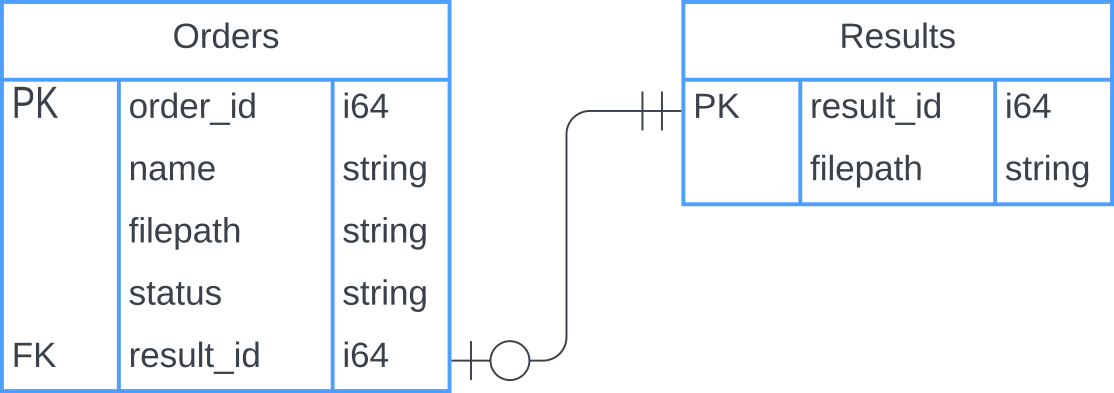
\includegraphics[width=\textwidth]{tex/pictures/app/database.png}
                \end{center}
                \caption{
                    Schemat bazy danych aplikacji przeglądarkowej.
                }\label{Picture:App:Database}
            \end{figure}

    % ===== ===== ===== =====
    % METODY
    % ===== ===== ===== =====
    \subsection{Metody grupowania sekwencji}

        W pracy zaimplementowano trzy metody grupowania sekwencji DNA. Każda metoda składa się z wyznaczania niepodobieństwa między sekwencjami DNA, które służą do budowy macierzy niepodobieństwa, a następnie do przeprowadzenia grupowania sekwencji. Każda z metod obejmuje:

        \begin{itemize}
            \item {wyznaczenie niepodobieństwa między sekwencjami,}
            \item {budowę macierzy niepodobieństwa,}
            \item {zastosowanie algorytmu grupowania.}
        \end{itemize}

        Budowanie macierzy niepodobieństwa oraz zastosowanie algorytmu grupowania wygląda we wszystkich metodach jednakowo. W dalszych sekcjach opisany zostanie proces wyznaczania niepodobieństwa między sekwencjami w zaimplementowanych metodach.
        
        \subsubsection{Zmodyfikowany algorytm Needlemana-Wunscha}

            Pierwszą metodą zastosowaną do wyznaczenia niepodobieństwa między sekwencjami DNA jest  zmodyfikowany algorytm Needlamana-Wunscha. Algorytm ten pierwotnie służy do globalnego wyrównania sekwencji genetycznych. Korzystajac z własności algorytmu, że w komórce $D_{n, m}$ macierzy podobieństwa budowanej przez algorytm znajduje się jakość globalnego wyrównania, dokonano modyfikacji algorytmu oraz odpowiedniego ustawienia parametrów, aby wynik ten odpowiadał mierze niepodobieństwa między sekwencjami. Modyfikacje te polegały na zmianie budowy macierzy podobieństwa oraz wprowadzeniu dodatkowych ograniczeń, w celu zapewnienia, że wartość w $D_{n, m}$ będzie zawierała się w przedziale $[0, \infty)$. Szczegóły wprowadzonych zmian względem wyrażenia \eqref{Equation:NeedlemanWunsch} przedstawiono poniżej:

            \begin{equation}
                \begin{aligned}
                    D_{i,j} &= \min
                    \begin{cases}
                    D_{i - 1, j} + g \\
                    D_{i, j - 1} + g \\
                    D_{i - 1, j - 1} + s(A_i, B_j)
                    \end{cases}, & \text{dla } & i \in \left(0, n\right] \text{ oraz } j \in \left(0, m\right] \\
                    & g, s(A_i, B_j) \in \mathbb{R}^{+}
                \end{aligned}
            \end{equation}

            gdzie,
            \begin{align*} 
                A, B -& \text{porównywane sekwencje}, \\
                n, m -& \text{długości sekwencji } A \text{ oraz } B, \\
                D -& \text{macierz podobieństwa o rozmiarach } n \text{ x } m, \\
                g -& \text{kara za przerwę}, \\
                s(A_i, B_j) -& \text{podobieństwo między  } i\text{-tym elementem w sekwencji A,} \\ 
                & \text{a } j \text{-tym elementem w sekwencji B}. \\
            \end{align*}

            Przyjęto wartości parametrów:
            \begin{align*}
                g &= 2, \\
                s(a, b) &= \begin{cases}
                    0, & \text{dla } a = b, \\
                    1, & \text{dla } a \neq b.
                \end{cases}
            \end{align*}

            Pełny przebieg metody przedstawiono na schemacie~\ref{Picture:Cluster:NeedlemanWunsch}. Czerwonym obramowaniem oznaczono krok, w którym wykorzystywany jest zmodyfikowany algorytm Needlemana-Wunscha.

            \question{
                Czy warto i stosowne jest pokazanie tutaj przykładu na przykładowych bardzo prostych danych?
            }

            \begin{figure}
                \begin{center}
                    {
% ===== BEGIN =====
% ----- -----
% COLORS
% ----- -----
\definecolor{Green}{HTML}{1dd1a1}
\definecolor{Blue}{HTML}{54a0ff}
\definecolor{Yellow}{HTML}{feca57}
\definecolor{Purple}{HTML}{5f27cd}
\definecolor{Grey}{HTML}{576574}
\definecolor{Red}{HTML}{ff6b6b}
\definecolor{Pink}{HTML}{ff9ff3}
\definecolor{Background}{HTML}{c8d6e5}

% ----- -----
% ELEMENTS
% ----- -----
\tikzstyle{Circle} = [circle, minimum size=1cm, line width=2pt, draw=black]
\tikzstyle{Box} = [rectangle, minimum width=10cm, minimum height=1.5cm, line width=2pt, text centered, inner sep=10pt, draw=black]
\tikzstyle{Arrow} = [very thick, -Triangle]
\tikzstyle{Arrow:Text} = [pos=0.5, right, font=\footnotesize]

% ----- -----
% PICTURE
% ----- -----
\begin{tikzpicture}[node distance=3cm]
    \node (input) [Circle] { Wejście };
    \node (distance) [Box, below of=input, align=center, draw=Red] { 1. Obliczenie niepodobieństwa między sekwencjami \\ \textbf{za pomocą algorytmu Needlemana-Wunscha} };
    \node (matrix) [Box, below of=distance] { 2. Stworzenie macierzy niepodoobieństwa };
    \node (cluster) [Box, below of=matrix, align=center] { 3. Grupowanie sekwencji \\ \textbf{za pomocą algorytmu k-medoidów}};
    \node (output) [Circle, below of=cluster] { Wyjście };

    \draw [Arrow] (input) -- (distance) node [Arrow:Text] {Zbiór sekwencji DNA};
    \draw [Arrow] (distance) -- (matrix) node [Arrow:Text] {Niepodobieństwo sekwencji};
    \draw [Arrow] (matrix) -- (cluster) node [Arrow:Text] {Macierz niepodobieństwa};
    \draw [Arrow] (cluster) -- (output) node [Arrow:Text] {Grupy};
\end{tikzpicture}

% ===== END =====
}
                \end{center}
                \caption{
                    Grupowanie sekwencji z wykorzystaniem zmodyfikowanego algorytmu Needlemana-Wunscha do określenia niepodobieństwa między sekwencjami.
                }\label{Picture:Cluster:NeedlemanWunsch}
            \end{figure}

        \subsubsection{Metoda zanurzeń \textit{k-merów}}
            Metoda zanurzeń \textit{k-merów} jest drugą klasyczną metodą wyznaczania niepodobieństwa między sekwencjami genetycznymi, w tym sekwencjami DNA. Polega ona na wyznaczeniu wszystkich \textit{k-merów} dla sekwencji wejściowych, a następnie obliczeniu niepodobieństwa sekwencji poprzez porównanie liczby wystąpień danych \textit{k-merów} w porównywanych sekwencjach.

            Z wyznaczonych \textit{k-merów} tworzy się wektor zanurzeń, w którym każda pozycja odpowiada określonemu \textit{k-merowi}. Przykładowo, dla \textit{k} = 2 (k-mery dwuznakowe) możemy przypisać odpowiednią pozycję w wektorze do każdego możliwego k-meru, np.:
            
            \[
            \text{AA} \to 0, \quad \text{AC} \to 1, \quad \text{AT} \to 2, \quad \text{AG} \to 3, \quad \text{CA} \to 4, \quad \dots
            \]
            
            Wektor zanurzeń dla danej sekwencji DNA zawiera liczbę wystąpień każdego \textit{k-meru} w odpowiednich pozycjach. Na przykład, dla sekwencji `AAACA' wektor zanurzeń dla $k=2$ może wyglądać następująco:
            
            \[
            \text{AATC} \to [2, 1, 0, 0, 1, \dots]
            \]
            
            gdzie liczba na pozycji 0 oznacza liczbę wystąpień \textit{AA} w sekwencji, liczba na pozycji 1 oznacza liczbę wystąpień \textit{AC}, itd. Następnie, na podstawie tych wektorów zanurzeń, oblicza się niepodobieństwo między sekwencjami, porównując ich wektory zanurzeń według wzoru:

            \begin{equation}
                dissimilarity_{kmer}(A, B, k) = \sqrt{\sum_{m \in M_{k}} (A_m - B_m)^{2}}
            \end{equation}

            gdzie,
            \begin{align*} 
                k -& \text{długość $k$-merów}, \\
                A, B -& \text{porównywane sekwencje}, \\
                M -& \text{zbiór wszystkich możliwych sekwencji genetycznych o długości $k$}, \\
                A_j, B_j -& \text{liczba wystąpień sekwencji } j \text{ odpowiednio w sekwencjach } A \text{ i } B. \\
            \end{align*}

            Pełny przebieg wykorzystania metody zanurzeń \textit{k-merów} w grupowaniu sekwencji został pokazany na schemacie~\ref{Picture:Cluster:KMer}. Czerwonym obramowaniem oznaczono krok, w którym wykorzystana została metoda.

            \question{
                Czy warto i stosowne jest pokazanie tutaj przykładu na przykładowych bardzo prostych danych?
            }

            \begin{figure}
                \begin{center}
                    {
% ===== BEGIN =====
% ----- -----
% COLORS
% ----- -----
\definecolor{Green}{HTML}{1dd1a1}
\definecolor{Blue}{HTML}{54a0ff}
\definecolor{Yellow}{HTML}{feca57}
\definecolor{Purple}{HTML}{5f27cd}
\definecolor{Grey}{HTML}{576574}
\definecolor{Red}{HTML}{ff6b6b}
\definecolor{Pink}{HTML}{ff9ff3}
\definecolor{Background}{HTML}{c8d6e5}

% ----- -----
% ELEMENTS
% ----- -----
\tikzstyle{Circle} = [circle, minimum size=1cm, line width=2pt, draw=black]
\tikzstyle{Box} = [rectangle, minimum width=10cm, minimum height=1.5cm, line width=2pt, text centered, inner sep=10pt, draw=black]
\tikzstyle{Arrow} = [very thick, -Triangle]
\tikzstyle{Arrow:Text} = [pos=0.5, right, font=\footnotesize]

% ----- -----
% PICTURE
% ----- -----
\begin{tikzpicture}[node distance=3cm]
    \node (input) [Circle] { Wejście };
    \node (embed) [Box, below of=input, draw=Red] { 1. Stworzenie zanurzeń k-merów };
    \node (distance) [Box, below of=embed, align=center] { 2. Obliczenie niepodobieństwa \\ między wektorami zanurzeń };
    \node (matrix) [Box, below of=distance] { 3. Stworzenie macierzy niepodoobieństwa };
    \node (cluster) [Box, below of=matrix, align=center] { 4. Grupowanie sekwencji \\ \textbf{za pomocą algorytmu k-medoidów}};
    \node (output) [Circle, below of=cluster] { Wyjście };

    \draw [Arrow] (input) -- (embed) node [Arrow:Text] {Zbiór sekwencji DNA};
    \draw [Arrow] (embed) -- (distance) node [Arrow:Text] {Wektory zanurzeń};
    \draw [Arrow] (distance) -- (matrix) node [Arrow:Text] {Niepodobieństwo sekwencji};
    \draw [Arrow] (matrix) -- (cluster) node [Arrow:Text] {Macierz niepodobieństwa};
    \draw [Arrow] (cluster) -- (output) node [Arrow:Text] {Grupy};
\end{tikzpicture}

% ===== END =====
}
                \end{center}
                \caption{
                    Grupowanie sekwencji z wykorzystaniem zanurzeń \textit{k-merów} do określenia niepodobieństwa między sekwencjami.
                }\label{Picture:Cluster:KMer}
            \end{figure}

        \subsubsection{Sieć neuronowa}

            Nową zaproponowaną metodą jest wykorzystanie sztucznej sieci neuronowej do redukcji wymiarowości wejściowych sekwencji DNA do postaci wektora cech o wymiarze $\mathbb{R}^{64}$. Sieć neuronowa wykorzystuje uczenie kontrastowe\cite{}, która umożliwia naukę reprezentacji danych wejściowych z zachowaniem właśności podobieństwa oraz niepodobieństwa między wejściowymi sekwencjami. Niepodobieństwo między sekwencjami zostanie obliczone poprzez obliczenie niepodobieństwa kosinusowego wyrażonego wzorem~\eqref{Equation:CosineDissimilarity} między wektorami cech sekwencji DNA.

            \paragraph{Architektura}
                Architektura modelu sieci neuronowej składa się z dwóch bloków splotowych zbudowanych z warstwy splotowej oraz normalizacji wsadowej, które odpowiadają za ekstrakcję niskopoziomowych cech sekwencji, warstwy spłaszczającej oraz trzech warstw perceptronów wielowarstwowych, które wykorzystują funkcję aktywacji GELU\cite{GELU} z wyłączeniem ostatniej warstwy. Wyjściem całego modelu jest wektor cech o wymiarze $\mathbb{R}^{64}$. 

                Schematycznie architektura została przedstawiona na rysunku~\ref{Picture:NeuralModel}. 

                \begin{figure}
                    \begin{center}
                        {
% ===== BEGIN =====
% ----- -----
% COLORS
% ----- -----
\definecolor{Green}{HTML}{1dd1a1}   % Input
\definecolor{Blue}{HTML}{54a0ff}    % Linear
\definecolor{Yellow}{HTML}{feca57}  % Convolution
\definecolor{Purple}{HTML}{5f27cd}  % Batch Norm
\definecolor{Grey}{HTML}{576574}    % Dropout
\definecolor{Red}{HTML}{ff6b6b}     % Output
\definecolor{Pink}{HTML}{ff9ff3}    % Activation
\definecolor{Background}{HTML}{c8d6e5}

% ----- -----
% ELEMENTS
% ----- -----
\tikzstyle{box} = [rectangle, rounded corners, minimum width=5cm, minimum height=1cm, text centered, draw=black, align=center]
\tikzstyle{input} = [box, fill=Green!30]
\tikzstyle{linear} = [box, fill=Blue!30]
\tikzstyle{conv} = [box, fill=Yellow!30]
\tikzstyle{bn} = [box, fill=Purple!30]
\tikzstyle{activation} = [box, fill=Pink!30]
\tikzstyle{dropout} = [box, fill=Grey!30]
\tikzstyle{output} = [box, fill=Red!30]

\tikzstyle{arrow} = [very thick, -Triangle]
\tikzstyle{arrow:text} = [pos=0.5, right, font=\footnotesize]

% ----- -----
% PICTURE
% ----- -----
\begin{tikzpicture}[node distance=2cm]
    \node (input) [input] { Wejście };
    \node (conv1) [conv, below of=input] { Splot 1D \\ \textbf{16@1x16, krok: 4} };
    \node (bn1) [bn, below of=conv1] { Normalizacja wsadowa };
    \node (conv2) [conv, below of=bn1] { Splot 1D \\ \textbf{32@1x8} };
    \node (bn2) [bn, below of=conv2] { Normalizacja wsadowa };
    \node (flatten) [linear, below of=bn2] { Warstwa spłaszczająca };
    \node (flatten-right) [right of=flatten, xshift=2cm] {};
    
    \node (fc1-left) [right of=input, xshift=2cm] {};
    \node (fc1) [linear, right of=input, xshift=6cm] { Warstwa gęsta };
    \node (act1) [activation, below of=fc1] { Aktywacja \\ \textbf{GELU} };
    \node (drop1) [dropout, below of=act1] { Wyłączenie neuronów };
    \node (fc2) [linear, below of=drop1] { Warstwa gęsta };
    \node (act2) [activation, below of=fc2] { Aktywacja \\ \textbf{GELU} };
    \node (drop2) [dropout, below of=act2] { Wyłączenie neuronów };
    \node (fc3) [linear, below of=drop2] { Warstwa gęsta };
    \node (output) [output, below of=fc3] { Wyjście };

    \draw [arrow] (input) -- (conv1) node [arrow:text] {1x600};
    \draw [arrow] (conv1) -- (bn1) node [arrow:text] {16x147};
    \draw [arrow] (bn1) -- (conv2) node [arrow:text] {16x147};
    \draw [arrow] (conv2) -- (bn2) node [arrow:text] {32x140};
    \draw [arrow] (bn2) -- (flatten) node [arrow:text] {32x140};

    \draw [arrow] (flatten.east) -- (flatten-right) -- node [arrow:text] {1x4480} (fc1-left) -- (fc1.west);
    \draw [arrow] (fc1) -- (act1) node [arrow:text] {1x4096};
    \draw [arrow] (act1) -- (drop1) node [arrow:text] {1x4096};
    \draw [arrow] (drop1) -- (fc2) node [arrow:text] {1x4096};
    \draw [arrow] (fc2) -- (act2) node [arrow:text] {1x512};
    \draw [arrow] (act2) -- (drop2) node [arrow:text] {1x512};
    \draw [arrow] (drop2) -- (fc3) node [arrow:text] {1x512};
    \draw [arrow] (fc3) -- (output) node [arrow:text] {1x64};
\end{tikzpicture}

% ===== END =====
}
                    \end{center}
                    \caption{
                        Schemat architektury sieci neuronowej.
                    }\label{Picture:NeuralModel}
                \end{figure}

            \paragraph{Dane wejściowe}
                Wejściem modelu są sekwencje DNA o długości $150$, które są kodowane do postaci wektora o wymiarach $1x600$ za pomocą kodu 1 z n\cite{Kod1zN}.

            \paragraph{Przykłady uczące}
                Przykłady uczące oraz walidacyjne składają się z kotwicy (ang. \textit{anchor}), sekwencji pozytywnej (ang. \textit{positive}) czyli podobnej do kotwicy oraz sekwencji negatywnej (ang. \textit{negative}) niepodobnej do kotwicy.
            
            \paragraph{Zbiór danych}
                Zbiór danych uczących oraz walidacyjnych został stworzony na podstawie zbioru \textit{CAMI II Toy Human Microbiome Project}\cite{Fritz2019}, dokładnie na podstawie pierwszej próbki sekwencji genetycznych, która zawiera symulowane dane metagenomiczne z mikrobiomu skóry człowieka. Przykłady uzyskano poprzez losowanie kotwic ze zbioru oraz modyfikację kotwic w celu uzyskania sekwencji pozytywnej oraz negatywnej w stopniu odpowiednio $[0; 0.2]$, $[0.2; 0.8]$. Modyfikacja polegała na zamianie punktowej danej zasady na inną.

            \paragraph{Funkcja straty}
                Wykorzystano funkcję straty zdefiniowaną jako:

                \begin{equation}
                    \text{Strata kontrastowa} = [m_{pos} - s_{pos}]_{+} + [s_{neg} - m_{neg}]_{+}
                \end{equation}

                gdzie,
                \begin{align*}
                    m_{pos}, m_{neg} &- \text{margines podobieństwa między przykładami pozytywnymi a kotwicą,} \\
                    &\text{oraz między przykładami negatywnymi a kotwicą}, \\
                    s_{pos}, s_{neg} &- \text{podobieństwo kosinusowe przykładu pozytywnego do kotwicy,} \\
                    &\text{oraz negatywnego do kotwicy.}
                \end{align*}

            \paragraph{Proces uczenia}
                Proces uczenia modelu sieci neuronowej został przeprowadzony na zbiorze $10^{6}$ przykładów uczących oraz $10^{4}$ przykładów walidacyjnych. 
                W procesie wykorzystano optymalizator \textit{AdamW}\cite{Loshchilov2017DecoupledWD} z wykładniczym spadkiem współczynnika uczenia oraz zanikiem wag (ang. \textit{weight decay}).
            
            \paragraph{Miara jakości}
                Jako miarę jakości wykorzystano stratę kontrastową modelu obliczoną na zbiorze walidacyjnym.

            \paragraph{Parametry procesu uczenia}
                Funkcja straty została wykorzystana z parametrami $m_{pos} = 1.0$, $m_{neg} = 0.25$.
                Przeprowadzono eksperymenty w celu określenia optymalnych parametrów sieci neuronowej. Sprawdzano parametry współczynnika uczenia $\lambda$, zaniku wag $w$, współczynnika $\gamma$ stosowanego w wykładniczym spadku współczynnika uczenia, parametr wyłączania neuronów oraz stosowność trzech warstw perceptronów wielowarstwowych. 
                W wyniku eksperymentów wybrano najlepsze parametry: $\lambda = 10^{-6}$, $w = $, $\gamma=0.99999$, współczynnik wyłączenia neuronów na poziomie $0.5$ oraz stwierdzono pozytywny wpływ zastosowania trzech warstw perceptronów. 

            Pełne wykorzystanie sztucznej sieci neuronowej w grupowaniu sekwencji zostało przedstawione na rysunku~\ref{Picture:Cluster:Neural}. Czerwonym obramowaniem oznaczono element wykorzystujący sztuczną sieć neuronową.

            \begin{figure}
                \begin{center}
                    {
% ===== BEGIN =====
% ----- -----
% COLORS
% ----- -----
\definecolor{Green}{HTML}{1dd1a1}
\definecolor{Blue}{HTML}{54a0ff}
\definecolor{Yellow}{HTML}{feca57}
\definecolor{Purple}{HTML}{5f27cd}
\definecolor{Grey}{HTML}{576574}
\definecolor{Red}{HTML}{ff6b6b}
\definecolor{Pink}{HTML}{ff9ff3}
\definecolor{Background}{HTML}{c8d6e5}

% ----- -----
% ELEMENTS
% ----- -----
\tikzstyle{Circle} = [circle, minimum size=1cm, line width=2pt, draw=black]
\tikzstyle{Box} = [rectangle, minimum width=10cm, minimum height=1.5cm, line width=2pt, text centered, inner sep=10pt, draw=black]
\tikzstyle{Arrow} = [very thick, -Triangle]
\tikzstyle{Arrow:Text} = [pos=0.5, right, font=\footnotesize]

% ----- -----
% PICTURE
% ----- -----
\begin{tikzpicture}[node distance=3cm]
    \node (input) [Circle] { Wejście };
    \node (embed) [Box, below of=input, align=center, draw=Red] { 1. Otrzymanie wektorów cech \\ \textbf{za pomocą sieci neuronowej} };
    \node (distance) [Box, below of=embed, align=center] { 2. Obliczenie niepodobieństwa \\ między wektorami cech };
    \node (matrix) [Box, below of=distance] { 3. Stworzenie macierzy niepodoobieństwa };
    \node (cluster) [Box, below of=matrix, align=center] { 4. Grupowanie sekwencji \\ \textbf{za pomocą algorytmu k-medoidów}};
    \node (output) [Circle, below of=cluster] { Wyjście };

    \draw [Arrow] (input) -- (embed) node [Arrow:Text] {Zbiór sekwencji DNA};
    \draw [Arrow] (embed) -- (distance) node [Arrow:Text] {Wektory cech};
    \draw [Arrow] (distance) -- (matrix) node [Arrow:Text] {Niepodobieństwo sekwencji};
    \draw [Arrow] (matrix) -- (cluster) node [Arrow:Text] {Macierz niepodobieństwa};
    \draw [Arrow] (cluster) -- (output) node [Arrow:Text] {Grupy};
\end{tikzpicture}

% ===== END =====
}
                \end{center}
                \caption{
                    Schemat architektury sztucznej sieci neuronowej.
                }\label{Picture:Cluster:Neural}
            \end{figure}

    % ===== ===== ===== =====
    % WYKORZYSTANE NARZĘDZIA
    % ===== ===== ===== ===== 
    \subsection{Wykorzystane technologie, narzędzia oraz biblioteki}

        \subsubsection{Języki programowania}

            W pracy wykorzystano języki programowania Rust\cite{Rust} oraz Python\cite{Python}.
            
            Język Python był wykorzystywany w początkowych fazach rozwoju pracy jako narzędzie do prototypowania rozwiązania oraz w ostatecznej wersji pracy do stworzenia skryptów automatyzyjących niektóre czynności związane z nauką sieci neuronowej oraz do generowania wykresów. Został on wybrany ze względu na bogatą bibliotekę standardową, dostępność wielu bibliotek zewnętrznych oraz wieloplatformowość.
            
            Język Rust został użyty do stworzenia wszystkich aplikacji oraz programów. Wybrany został ze względu na wysokość wydajność, bezpieczne zarządzanie pamięcią oraz dużą dostępność bibliotek programistycznych, które można zainstalować za pomocą menedżera pakietów \textit{cargo}\cite{Rust:cargo} dołączonego wraz ze środowiskiem języka Rust. Dodatkowymi atutami, które przyczyniły się do wyboru języka, jest bogaty system typów oraz kompilacja do kodu maszynowego. 

        \subsubsection{Biblioteki programistyczne}

            Aplikację przeglądarkową zrealizowano z wykorzystaniem biblioteki \textit{axum}\cite{Rust:axum} opartej na asynchronicznym środowisku wykonawczym \textit{tokio}\cite{Rust:tokio} języka Rust.
            Do generowania zawartości stron w formacie HTML wykorzystano silnik szablonów \textit{askama}\cite{Rust:askama}. Komunikację z bazą danych zapewniła biblioteka \textit{sqlx}\cite{Rust:sqlx}. Użyto dodatkowo biblioteki \textit{dotenv}\cite{Rust:dotenv} w celu załadowania zmiennych środowiskowych z pliku, które niezbędne są do prawidłowego działania aplikacji.

            Aplikacja konsolowa została oparta na bibliotece \textit{clap}\cite{Rust:clap}, która pozwoliła na zdefiniowanie interfejsu użytkownika, w postaci dostępnych poleceń wraz z parametrami.

            Bibioteka \textit{exquisitor-core} korzysta z biblioteki \textit{kmedoids}\cite{Schubert:2022}, która implementuje grupowanie k-medoidów oraz bibliotek pomocniczych \textit{num-traits}, \textit{tempfiles} oraz \textit{float-cmp}, które wykorzystywane są w testach jednostkowych.

            Model sieci neuronowej został zbudowany przy użyciu biblioteki \textit{burn}\cite{Rust:burn} oraz silnika obliczeniowego \textit{wgpu}.

            Ponadto w obu aplikacjach oraz bibliotece wykorzystywana jest biblioteka \textit{serde}\cite{Rust:serde} umożliwiającą serializację i deserializację danych do różnych formatów oraz biblioteka \textit{rand}\cite{Rust:rand} zapewniająca generator liczb pseudolosowych.

        \subsubsection{Narzędzia}
            
            W pracy zostały wykorzystane następujące narzędzia:
            \begin{itemize}
                \item \textit{cargo} jako menedżer pakietów i system budowania w Rust,
                \item \textit{rustup} do automatycznego zarządzania wersjami Rust,
                \item \textit{clippy} do statycznej analizy kodu w Rust,
                \item \textit{rustfmt} do automatycznego formatowania kodu źródłowego w Rust,
                \item \textit{cargo test} do przeprowadzania testów jednostkowych,
                \item \textit{git} jako system kontroli wersji, umożliwiający śledzenie zmian oraz zarządzanie historią kodu.
            \end{itemize}

    % ===== ===== ===== =====
    % INTERFEJS UŻYTKOWNIKA + INSTRUKCJA UŻYTKOWNIKA
    % ===== ===== ===== =====
    \subsection{Interfejs użytkownika}

        \subsubsection{Opis interfejsu użytkownika}

            \paragraph{Aplikacja konsolowa}
                
                Aplikacja konsolowa działa w środowisku terminalowym i wykonuje polecenia wprowadzone przez użytkownika, generując komunikaty o różnych poziomach ważności.
                
                \begin{itemize}
                
                    \item{
                        \textbf{Polecenia aplikacji konsolowej:}
                        Polecenia w aplikacji konsolowej składają się z głównego polecenia oraz opcjonalnych argumentów. Główne polecenie jest zawsze wymaganym elementem, a argumenty mogą być opcjonalne lub obowiązkowe w zależności od głównego polecenia.
                        Przykładowe polecenie wygląda następująco:
                        \[
                            \texttt{./exquisitor-cli -\phantom{}-log-level INFO search -\phantom{}-input tmp.fasta}
                        \]
                        gdzie,
                        \begin{itemize}
                            \item {
                                \texttt{search} - główne polecenie aplikacji,
                            }
                            \item {
                                \texttt{-\phantom{}-log-level INFO} - argument ustawiający poziom ważności komunikatów na informacyjny,
                            }
                            \item {
                                \texttt{-\phantom{}-input tmp.fasta} - argument wskazujący plik wejściowy.
                            }
                        \end{itemize}
                        Ustawienie poziomu ważności komunikatów musi nastąpić przed podaniem głównego polecenia aplikacji. Domyślnie poziom ważności komunikatów jest ustawiony na informacyjny.
                    }
                    \item {
                        \textbf{Wykonanie polecenia:}
                        W wyniku wykonania polecenia przez aplikację użytkownik otrzymuje komunikat o błędzie lub sukcesie wykonania. W przypadku sukcesu komunikat wygląda następująco:
                        \texttt{Command executed successfully!}.
                    }
                    \item {
                        \textbf{Błędy i komunikaty systemowe:}
                        Aplikacja wyświetla komunikaty o błędach w przypadku nieprawidłowego użycia polecenia oraz wprowadzenia nieobsługiwanych argumentów. Typowe komunikaty o błędach mogą obejmować:
                        \begin{itemize}
                            \item {
                                \texttt{error: the following required arguments were not provided} – gdy użytkownik nie wprowadzi wszystkich wymaganych argumentów,
                            }
                            \item {
                                \texttt{error: unexpected argument <argument> found} – gdy użytkownik wprowadzi argument, który nie jest obsługiwany,
                            }
                            \item {
                                \texttt{Error: No such file or directory (os error 2)} – gdy użytkownik podał ścieżkę do pliku lub programu, który nie istnieje.
                            }
                        \end{itemize}
                    }
                    \item {
                        \textbf{Pomoc i instrukcje:}
                        Aplikacja posiada wbudowane polecenie \texttt{-\phantom{}-help}, które pozwala na wyświetlenie informacji o dostępnych poleceniach, ich opisach oraz wymaganych argumentach.
                        Aby uzyskać informacje o poleceniu \texttt{search}, użytkownik może wykorzystać następujące polecenie: 
                        \[
                            \texttt{./exquisitor-cli search --help}
                        \]
                        W wyniku wykonania tego polecenia, użytkownik otrzyma opis polecenia, przykładowe użycie oraz listę wszystkich argumentów wraz z ich opisami.
                    }

                \end{itemize}

            \paragraph{Aplikacja przeglądarkowa}
                Aplikacja przeglądarkowa działa w środowisku przeglądarki internetowej. Umożliwia zlecanie zadań klasyfikacji taksonomicznej oraz wyszukiwanie i przeglądanie wyników tych zleceń.

                \begin{itemize}
                    \item {
                        \textbf{Układ i elementy interfejsu:}
                        Aplikacja składa się z 4 ekranów użytkownika:
                        \begin{itemize}
                            \item {
                                \textbf{Strona główna} - na tym ekranie znajduje się lista dziesięciu ostatnio przeprowadzonych zleceń, formularz do wyszukiwania zleceń po nazwie lub identyfikatorze oraz przycisk do dodawania nowych zleceń. Jest to główny ekran aplikacji.
                                }
                            \item {
                                \textbf{Strona zlecenia} - ekran wyświetlający szczegóły konkretnego zlecenia, w tym identyfikator, opis, status, daty rozpoczęcia i zakończenia oraz wyniki.
                            }
                            \item {
                                \textbf{Strona dodania zlecenia} - ekran, na którym użytkownik może wprowadzić nowe zlecenie. 
                            }
                            \item {
                                \textbf{Ekran błędu} - ekran odpowiedzialny za wyświetlanie komunikatów o błędach
                            }
                        \end{itemize}
                        Na rysunku~\ref{Picture:App:WebScreen} znajduje się zrzut ekranu z głównego ekranu aplikacji przeglądarkowej.
                    }
                    \item {
                        \textbf{Formularze i przyciski:}
                        Aplikacja zawiera dwa formularze:
                        \begin{itemize}
                            \item {
                                \textbf{Formularz wyszukiwania eksperymentu} - pozwala na znalezienie eksperymentu przez podanie jego nazwy lub identyfikatora.
                            }
                            \item {
                                \textbf{Formularz dodania zlecenia} - pozwala na dodanie nowego zlecenia klasyfikacji taksonomicznej poprzez podanie nazwy, opisu oraz pliku z danymi wejściowymi.
                            }
                        \end{itemize}
                    }
                    \item {
                        \textbf{Komunikaty:}
                        Aplikacja wyświetla komunikaty o błędach, w przypadku ich wystąpienia. Działania zakończone sukcesem nie generują komunikatów.
                    }
                \end{itemize}

                \begin{figure}
                    \begin{center}
                        \todo{
    Tutaj powinien być zrzut ekranu z aplikacji przeglądarkowej.
}
                    \end{center}
                    \caption{
                        Ekran główny aplikacji przeglądarkowej.
                    }\label{Picture:App:WebScreen}
                \end{figure}

        \subsubsection{Instrukcja użytkownika}

            Niniejsza instrukcja użytkownika zawiera szczegółowy opis procesu instalacji, uruchamiania oraz użytkowania aplikacji konsolowej i przeglądarkowej. W pierwszej części omówiono proces instalacji wymaganego środowiska, a w kolejnych sekcjach przedstawiono szczegółowe instrukcje użytkownika dla obu rodzajów aplikacji.

            \paragraph{Wymagania techniczne:}
                \begin{itemize}
                    \item {
                        \textbf{System operacyjny:} Ubuntu 20.0 lub nowszy.
                    }
                    \item {
                        \textbf{Pamięć RAM:} minimum 4 GB, zalecane 8 GB.
                    }
                    \item {
                        \textbf{Karta graficzna:} Nvidia GeForce GTX 1060 6 GB lub lepsza.
                    }
                    \item {
                        \textbf{Miejsce na dysku:} minimum 1 TB dostępnej przestrzeni.
                    }
                \end{itemize}

            \paragraph{Instalacja \texttt{blastn} oraz bazy danych nukleotydów \texttt{nt}}

                \begin{enumerate}
                    \item {
                        Skopiuj skrypt instalacyjny o nazwie \texttt{download\_database.sh} do środowiska, w którym będzie przeprowadzana instalacja.
                    }
                    \item {
                        Nadaj skryptowi odpowiednie uprawnienia do wykonania, używając polecenia: \texttt{sudo chmod +x download\_database.sh}.
                    }
                    \item {
                        Uruchom skrypt, aby rozpocząć pobieranie i instalację \texttt{blastn} oraz bazy danych nukleotydów \texttt{nt}: \texttt{sudo ./download\_database.sh}.
                    }
                    \item {
                        Skrypt automatycznie pobierze, zainstaluje oraz rozpakuje aplikację \texttt{blastn} oraz bazę danych nukleotydów \texttt{nt}.
                    }
                \end{enumerate}

            \paragraph{Instalacja wymaganych programów:}

                \begin{enumerate}
                    \item {
                        Zainstaluj pakiet \texttt{git} za pomocą polecenia: \texttt{sudo apt install git}.
                    }
                    \item {
                        Zainstaluj środowisko języka Rust\footnote{Instrukcje instalacji języka Rust dostępne są pod adresem: \texttt{https://www.rust-lang.org/tools/install}.}.
                    }
                \end{enumerate}

            \paragraph{Kompilacja aplikacji}
                
                \begin{enumerate}
                    \item {
                        Pobierz repozytorium rozwiązania za pomocą polecenia \texttt{git clone <url>}, gdzie \texttt{<url>} jest adresem repozytorium z kodem.
                    }
                    \item {
                        Przejdź do folderu \texttt{exquisitor/exquisitor-app} oraz uruchom następujące polecenia:

                        \begin{itemize}
                            \item {
                                \texttt{sqlx database create -\phantom{}-database-url sqlite://exquisitor.db}
                            }
                            \item {
                                \texttt{sqlx migrate run -\phantom{}-database-url sqlite://exquisitor.db}
                            }
                        \end{itemize}
                    }
                    \item {
                        Przejdź do folderu \texttt{exquisitor}, oraz uruchom polecenie \texttt{cargo build -\phantom{}-release -\phantom{}-bins}.
                    }
                    \item {
                        Aplikacja konsolowa oraz przeglądarkowa powinny być skompilowane i znajdują się w folderze \texttt{exquisitor/target/release}. 
                        Skopiuj pliki wykonywalne aplikacji do docelowej lokacji.
                    }
                    \item{
                        Skopiuj plik \texttt{exquisitor.db} z folderu \texttt{exquisitor/exquisitor-app} do tej samej lokacji co aplikacja przeglądarkowa.
                    }
                \end{enumerate}
            
            \paragraph{Uruchomienie aplikacji konsolowej}

                \begin{enumerate}
                    \item {
                        Przejdź do folderu, w którym znajduje się plik wykonywalny aplikacji konsolowej.
                    }
                    \item {
                        Ustaw zmienne środowiskowe \texttt{BLASTDB} oraz \texttt{BLASTN}, aby wskazywały odpowiednio na folder z bazą danych nukleotydów oraz na program \texttt{blastn}. 
                        W przypadku standardowej instalacji środowiska za pomocą skryptu \texttt{download\_database.sh} zmienne należy ustawić odpowiednio na \texttt{/blast/db} oraz \texttt{/blast/executables/bin/blastn}.
                    }
                    \item {
                        Aplikacja konsolowa jest gotowa do użycia. Możliwe jest uruchomienie dowolnego polecenia z tabeli~\ref{Table:ConsoleCommands}. Szczegóły dotyczące składni poleceń oraz argumentów znajdują się w tabeli~\ref{Table:ConsoleCommandsSyntax}.
                    }
                \end{enumerate}

                \begin{table}[!ht] \centering
                    \caption{Polecenia aplikacji konsolowej.}\label{Table:ConsoleCommands}

                    \begin{tabularx}{\textwidth}{| >{\footnotesize}m{0.25\textwidth} |  >{\footnotesize}X |} 
                        \hline
                        \textbf{\normalsize Polecenie}  & \textbf{\normalsize Opis polecenia} \\ \hline \hline
                        \texttt{experiment} 	        & Uruchamia wskazane polecenie jako eksperyment. Pozwala na monitorowanie wykorzystania procesora oraz pamięci RAM oraz ograniczenie trwania eksperymentu. \\ \hline
                        \texttt{compare}		        & Porównuje dwa zestawy wyników klasyfikacji taksonomicznej, jako wynik zwraca jakość względną między nimi. \\ \hline
                        \texttt{compare-clusters} 	    & Porównuje dwa zestawy grup otrzymanych za pomocą algorytmu grupowania, jako wynik zwraca jakość grupowania. \\ \hline
                        \texttt{search}                 & Wyszukuje sekwencje DNA w bazie danych bez uruchamiania pełnego potoku przetwarzania. \\ \hline
                        \texttt{run}		            & Uruchamia pełną klasyfikację taksonomiczną z wykorzystaniem potoku przetwarzania. \\ \hline
                    \end{tabularx}
                
                \end{table}

            \paragraph{Przykładowe wykorzystanie aplikacji konsolowej}

                \todo{
                    uruchomienie wyszukiwania oraz przykład wyniku
                }

            \paragraph{Uruchomienie aplikacji przeglądarkowej}

                \begin{enumerate}
                    \item {
                        Przejdź do folderu, w którym znajduje się plik wykonywalny aplikacji przeglądarkowej.
                    }
                    \item {
                        Uruchom plik wykonywalny za pomocą polecenia: \texttt{./exquisitor-app}.
                    }
                    \item {
                        Aplikacja powinna się uruchomić. Interfejs użytkownika dostępny jest pod adresem: 
                        \texttt{localhost:3000}.
                    }
                \end{enumerate}

            \paragraph{Przykładowe wykorzystanie aplikacji przeglądarkowej}

                \todo{
                    dodanie eksperymentu / wyświetlenie wyniku
                }

                \begin{longtblr}[
                    caption = {Składnia poleceń aplikacji konsolowej.},
                    label = {Table:ConsoleCommandsSyntax}
                ]{
                    colspec = {| >{\footnotesize}m{0.2\textwidth} | >{\footnotesize}m{0.2\textwidth} | >{\footnotesize}X |},
                    rowhead = 1,
                }
                    \hline
                    \textbf{\normalsize Polecenie}     & \textbf{\normalsize Argument}    & \textbf{\normalsize Opis argumentu} \\*
                    \hline \hline

                    \multirow{4}{*}{\texttt{experiment}}  & \texttt{-\phantom{}-resolution <liczba>}   & Rozdzielczość monitorowania eksperymentu w sekundach. Określa jak często będzie sprawdzane wykorzystanie zasobów przez eksperyment oraz przekroczenie czasu trwania eksperymentu. \\*
                                                          & \texttt{-\phantom{}-command <polecenie>}   & Polecenie, które zostanie wykonane jako eksperyment. Powinno to był poprawne polecenie aplikacji konsolowej. \\*
                                                          & \texttt{-\phantom{}-output <ścieżka>}      & Ścieżka do pliku, w którym zostaną zapisane wyniki monitorowania eksperumentu. Wyniki zapisywane są jako tabela w formacie CSV. \\*
                                                          & \texttt{-\phantom{}-max-duration <liczba>} & Maksymalny czas trwania eksperymentu w sekundach. Po przekroczeniu czasu trwania eksperymentu nastąpi jego przerwanie. \\ \hline

                    % % compare             & \texttt{
                            
                    % % } \\ \hline % @TODO

                    \multirow{3}{*}{\texttt{compare-clusters}}  & \texttt{-\phantom{}-reference <ścieżka>} & Ścieżka do pliku z wynikami klasyfikacji taksonomicznej, które stanowią punkt odniesienia w porównaniu. \\*
                                                                & \texttt{-\phantom{}-second <ścieżka>}    & Ścieżka do pliku z wynikami klasyfikacji taksonomicznej, które zostaną porównane względem wskazanych wyników referencyjnych. \\*
                                                                & \texttt{[-\phantom{}-output <ścieżka>]}  & Ścieżka do pliku, w którym zostaną zapisane wyniki dokonanego porównania. \\ \hline

                    \multirow{4}{*}{\texttt{search}}    & \texttt{-\phantom{}-input <ścieżka>}    & Ścieżka do pliku, który zawiera sekwencje DNA. \\*
                                                        & \texttt{-\phantom{}-output <ścieżka>}   & Ścieżka do pliku, w którym zostaną zapisane wyniki wyszukiwania. \\*
                                                        & \texttt{-\phantom{}-blast <ścieżka>}    & Ścieżka do pliku wykonywalnego \texttt{blastn}. \\*
                                                        & \texttt{-\phantom{}-blast-db <ścieżka>} & Ścieżka do folderu z bazą danych nukleotydów \texttt{nt}. \\ \hline

                    \multirow{13}{*}{\texttt{run}}      & \texttt{-\phantom{}-input <ścieżka>}           & Ścieżka do pliku, który zawiera sekwencje DNA. \\*
                                                        & \texttt{-\phantom{}-output <ścieżka>}          & Ścieżka do pliku, w którym zostaną zapisane wyniki klasyfikacji taksonomicznej. \\*
                                                        & \texttt{-\phantom{}-file-format <file-format>} & Format pliku z sekwencjami DNA. Dostępne formaty: \texttt{fasta}, \texttt{fastq} oraz \texttt{auto} (automatyczne wykrywanie formatu na podstawie rozszerzenia pliku). \\*
                                                        & \texttt{-\phantom{}-pipeline <pipeline>}       & Metoda wykorzystana do określania niepodobieństwa między sekwencjami DNA. Dostępne metody: \texttt{basic} (zmodyfikowany algorytm Needlemana-Wunscha), \texttt{k-mer} (zanurzenia k-merów), \texttt{neural} (sieć neuronowa). \\*
                                                        & \texttt{-\phantom{}-cluster <cluster>}         & Algorytm grupowania. Dostępne algorytmy: \texttt{k-medoid}. \\*
                                                        & \texttt{-\phantom{}-k <liczba>}                & Liczba grup tworzonych przez algorytm grupowania. \\*
                                                        & \texttt{-\phantom{}-blast <ścieżka>}           & Ścieżka do pliku wykonywalnego \texttt{blastn}. \\*
                                                        & \texttt{-\phantom{}-blast-db <ścieżka>}        & Ścieżka do folderu z bazą danych nukleotydów \texttt{nt}. \\*
                                                        & \texttt{[-\phantom{}-gap-penalty <liczba>]}    & Parametr kary za przerwę w metodzie z wykorzystaniem zmodyfikowanego algorytmu Needlemana-Wunscha. Argument obowiązkowy przy podaniu \texttt{basic} jako wartości argumentu \texttt{-{}-pipeline}. \\*
                                                        & \texttt{[-\phantom{}-kmer <ścieżka>]}          & Długość wykorzystanych k-merów w metodzie zanurzeń k-merów. Argument obowiązkowy przy podaniu \texttt{k-mer} jako wartości argumentu \texttt{-{}-pipeline}. \\*
                                                        & \texttt{[-\phantom{}-model <ścieżka>]}         & Ścieżka do pliku, który zawiera zapisane wagi modelu sieci neuronowej. Argument obowiązkowy przy podaniu \texttt{neural} jako wartości argumentu \texttt{-{}-pipeline} .\\*
                                                        & \texttt{[-\phantom{}-only-cluster]}            & Flaga, której użycie powoduje przerwanie potoku przetwarzania po przeprowadzeniu grupowania sekwencji.  \\*
                                                        & \texttt{[-\phantom{}-save-clusters}            & Flaga, której użycie powoduje zapisanie wyników grupowania do pliku. \\ \hline
                \end{longtblr}

    % ===== ===== ===== =====
    % OPIS TESTÓW JEDNOSTKOWYCH
    % ===== ===== ===== =====
    \subsection{Testy}

        \subsubsection{Testy jednostkowe}

            Testy jednostkowe zostały przeprowadzone w celu weryfikacji poprawności działania poszczególnych funkcji i metod w izolacji. Testy obejmowały zarówno typowe scenariusze wykorzystania funkcjonalności, jak i potencjalne sytuacje błędne.
            
            \paragraph{Zakres}  
            Testy jednostkowe objęły większość funkcji oraz metod w bibliotece \texttt{exquisitor-core}. Szczególną uwagę poświęcono poprawności działania funkcji związanych z wczytywaniem sekwencji oraz obliczaniem miar.
            
            \paragraph{Narzędzia}  
            Wykorzystano wbudowane narzędzie \texttt{cargo test} języka Rust, do uruchamiania testów jednostkowych. Narzędzie to automatycznie uruchamia testy zawarte w plikach implementacyjnych, traktując je jako testy jednostkowe.

            \paragraph{Pokrycie testami}
            Do sprawdzenia stopnia pokrycia kodu testami wykorzystano narzędzie \texttt{tarpaulin}\cite{Rust:tarpaulin}. 
            Osiągnięto \textbf{65\%} pokrycia linii kodu za pomocą testów jednostkowych.

        \subsubsection{Testy manualne}
        
            \paragraph{Zakres}
            Testy manualne objęły działanie interfejsu użytkownika aplikacji konsolowej oraz aplikacji przeglądarkowej. W przypadku aplikacji konsolowej sprawdzono działanie wszystkich poleceń z uwzględnieniem klasycznych sytuacji błędnych. W aplikacji przeglądarkowej testowano funkcjonalności: dodawania, wyszukiwania i przeglądania zleceń.

            \paragraph{Metoda}
            Ręczne wykonywanie scenariuszy testowych, takich jak:
            \begin{itemize}
                \item {Dodanie nowego zlecenia i weryfikacja czy wyświetla się na stronie głównej aplikacji przeglądarkowej.}
                \item {Wyszukanie dodanego zlecenia po identyfikatorze na stronie głównej.}
                \item {Uruchomienie polecenia aplikacji konsolowej wyszukiwania w bazie danych i sprawdzenie, czy powstał odpowiedni plik z wynikami.}
            \end{itemize}

\cleardoublepage
\section{Badanie jakości i wydajności zaproponowanego rozwiązania}

    W ramach pracy przeprowadzono eksperymenty polegające na porównaniu wydajności oraz jakości zaimplementowanych metod do grupowania sekwencji genetycznych w kontekście pełnej klasyfikacji taksonomicznej przeprowadzonej z wykorzystaniem potoku przetwarzania. W eksperymentach jako punkt odniesienia wybrano klasyfikację taksonomiczną wszystkich sekwencji wejściowych bez użycia potoku przetwarzania.

    % ===== ===== ===== =====
    % OPIS ŚRODOWISKA EKSPERYMENTALNEGO
    % ===== ===== ===== =====
    \subsection{Opis środowiska eksperymentalnego}

        Eksperymenty zostały przeprowadzone na maszynie wirtualnej wykorzystującej technologię KVM o specyfikacji podanej poniżej.

        % \subsubsection{Specyfikacja techniczna}\

            \begin{itemize}
                \item {
                    \textbf{System operacyjny:} Ubuntu 22.04 LTS.
                }
                \item {
                    \textbf{Procesor:} 4 rdzenie wirtualne procesora Intel Core i7-6850K.
                }
                \item {
                    \textbf{Pamięć RAM:} 40GB.
                }
                \item {
                    \textbf{Karta graficzna:} Nvidia GeForce GTX 1080 TI.
                }
                \item {
                    \textbf{Dysk:} dysk sieciowy 1 TB z prędkością odczytu 1 Gbps.
                }
                \item {
                    \textbf{Oprogramowanie:} pakiet \texttt{BLAST} w wersji 2.16.0 oraz sterowniki karty graficznej.
                }
            \end{itemize}

    % ===== ===== ===== =====
    % MIARA JAKOŚCI
    % ===== ===== ===== =====
    \subsection{Miara jakości}

        Jako miarę jakości klasyfikacji taksonomicznej wykorzystano zmodyfikowany indeks Jaccarda, wyrażony za pomocą wzoru~\ref{Equation:Quality}.

        \begin{equation}
            \text{Q} = \frac{
                \sum_{r \in (O(R) \cap O(E))} R_{r}
            }{
                \sum_{r \in (O(R) \cup O(E))} R_{r}
            }
            \label{Equation:Quality}
        \end{equation}

        gdzie:
        \begin{align*}
            R &- \text{zbiór wyników referencyjnych,} \\
            E &- \text{zbiór wyników otrzymanych,} \\
            R_{r} &- \text{liczba wyników w zbiorze referencyjnym przypisanych do organizmu $r$,} \\
            O(X) &- \text{zbiór unikalnych organizmów, dla których przypisano wyniki w zbiorze X. }
        \end{align*}

        Miara została wykorzystana do porównania jakości klasyfikacji taksonomicznej przeprowadzanej z wykorzystaniem zaimplementowanych metod względem klasyfikacji taksonomicznej bez użycia potoku przetwarzania.

        Do porównywania jakości wielu przebiegów klasyfikacji taksonomicznej wykorzystano średnią jakość ważoną zdefiniowaną za pomocą wzoru~\ref{Equation:WeightedAverageQuality}.

        \begin{equation}
            Q_{\text{avg}} = \sum_{c \in C} \frac{n_c}{n} Q_c
            \label{Equation:WeightedAverageQuality}
        \end{equation}

        gdzie:
        \begin{align*}
          C &- \text{zbiór wszystkich przebiegów klasyfikacji taksonomicznych,} \\
          Q_c &- \text{jakość klasyfikacji taksonomicznej $c$,} \\
          n_c &- \text{liczba sekwencji wejściowych do klasyfikacji taksonomicznej $c$,}\\
          n   &- \text{liczba sekwencji wejściowych $n = \sum_{c \in C} n_{c}.$}
        \end{align*}

        Wykorzystano również dodatkowe miary jakości, które zostały zastosowane do oceny jakości utworzonych grup przez potok przetwarzania. Pierwszą wykorzystaną miarą jest znormalizowana informacja wzajemna (ang. \textit{Normalized mutual information, NMI}) i służy do oceny jakości grup, drugą jest czułość (ang. \textit{sensitivity}), która wykorzystana jest do oceny reprezentantów grup. Miary zostały zdefiniowane odpowiednio wzorami \eqref{Equation:NMI} i \eqref{Equation:Sensitivity}.

        \begin{equation}
            NMI(X, Y) = \frac{I(X, Y)}{\sqrt{H(X) \cdot H(Y)}}
            \label{Equation:NMI}
        \end{equation}

        gdzie:
        \begin{align*}
            I(X, Y) &= \sum_{y \in Y}{ \sum_{x \in X}{p(x, y) \log_{2}{\frac{p(x, y)}{p(x) p(y)}}}}, \\
            H(X) &= - \sum_{x \in X}{ p(x) \log_{2}{p(x)}}, \\
            I(X, Y) &- \text{informacja wzajemna między zbiorami $X$ oraz $Y$}, \\
            H(X) &- \text{entropia zbioru $X$}, \\
            H(Y) &- \text{entropia zbioru $Y$}, \\
            p(x) &- \text{prawdopodobieństwo zajścia zdarzenia $x$}, \\
            p(x, y) &- \text{wspólny rozkład prawdopodobieństwa $X$ oraz $Y$ }.
        \end{align*}

        \begin{equation}
            sensitivity = \frac{\text{TP}}{
                \text{TP} + \text{TN}
            }
            \label{Equation:Sensitivity}
        \end{equation}

        gdzie:
        \begin{align*}
            TP &- \text{liczba wyników prawdziwie dodatnich,} \\
            TN &- \text{liczba wyników fałszywie ujemnych.}
        \end{align*}

        Dodatkowe miary jakości zostały wykorzystane do oceny jakości względnej między zaimplementowanymi metodami.

    % ===== ===== ===== =====
    % ZBIÓR DANYCH
    % ===== ===== ===== =====
    \subsection{Zbiór danych do badań}

        \subsubsection{Opis zbioru danych}

            W eksperymentach wykorzystano ten sam zbiór sekwencji genetycznych, co w uczeniu modelu sztucznej sieci neuronowej. Zbiór \textit{CAMI II Toy Human Microbiome Project}\cite{Fritz:2019} został wybrany, ponieważ został stworzony w celu oceny wydajności algorytmów bioinformatycznych oraz zawiera znaczną liczbę sekwencji genetycznych, co umożliwiło jego wykorzystanie go zarówno w eksperymentach, jak i w uczeniu modelu sztucznej sieci neuronowej.

            Na podstawie zbioru stworzono podzbiory sekwencji o rozmiarach wyrażonych wzorem $2^k$ dla $k \in [0, 12]$. Zbiory są rozłączne, a do ich budowy wykorzystano wyłącznie te sekwencje, które nie zostały użyte do uczenia modelu sztucznej sieci neuronowej.

        \subsubsection{Przygotowanie zbioru danych}

            Podzbiory powstały poprzez losowanie bez zwracania indeksów sekwencji genetycznych ze zbioru referencyjnego, które powinny trafić do podzbioru. W losowaniu wykorzystano informację o indeksach sekwencji wykorzystanych w zbiorze uczącym oraz walidacyjnym sztucznej sieci neuronowej. W celu umożliwienia dalszego wykorzystania zbioru danych zapisano do pliku indeksy sekwencji wykorzystanych w procesie budowy zbioru eksperymentalnego. Podzbiory sekwencji zostały zapisane do plików w formacie FASTA.

    % ===== ===== ===== =====
    % PROCEDURA PRZEPROWADZANIA EKSPERYMENTÓW
    % ===== ===== ===== =====
    \subsection{Procedura przeprowadzania eksperymentów}

        Eksperymenty zostały przeprowadzone za pomocą zaimplementowane polecenia aplikacji konsolowej \texttt{experiment}, które pozwala na nadzorowanie wykorzystania procesora oraz pamięci RAM przez polecenie, oraz kontrolowanie maksymalnego czasu trwania wykonywanego polecenia.

        Dane do obu eksperymentów zostały zgromadzone w wyniku przeprowadzenia klasyfikacji taksonomicznej z wykorzystaniem zaimplementowanych metod oraz klasyfikacji taksonomicznej bez wykorzystania potoku przetwarzania dla każdego podzbioru osobno.

        W wyniku przeprowadzonych klasyfikacji taksonomicznych otrzymano informację o przebiegu procesu w formie plików z rozszerzeniem \texttt{.experiment}, zawierających dane dotyczące wykorzystania zasobów podczas przebiegu klasyfikacji oraz czasu jej trwania. W przypadku sukcesu procesu grupowania otrzymano plik z rozszerzeniem \texttt{.clusters}, który zawiera informację o stworzonych grupach. Natomiast w przypadku pomyślnej klasyfikacji taksonomicznej końcowe wyniki całego procesu zapisano do pliku z rozszerzeniem \texttt{.search}.

        \subsubsection{Parametry}

            Maksymalny czas trwania jednej klasyfikacji taksonomicznej został ograniczony do 12 godzin. Dla wszystkich metod wybrano algorytm grupowania $k$-medoidów oraz określono liczbę tworzonych grup przez algorytm grupowania za pomocą wzoru $\sqrt{n}$, gdzie $n$ to liczba sekwencji wejściowych. W metodzie z wykorzystaniem zmodyfikowanego algorytmu Needlemana-Wunscha wykorzystano parametry określone w sekcji~\ref{Method:NeedlemanWunsch}. W przypadku metody wykorzystującej zanurzenia $k$-merów parametr $k$ został ustawiony na $4$. W metodzie z wykorzystaniem sztucznej sieci neuronowej wykorzystano wcześniej stworzony model.

        \subsubsection{Skrypty}

            Do przeprowadzenia eksperymentów zostały wykorzystane opracowane skrypty w języku \texttt{bash}. Każdy skrypt uruchamia klasyfikację taksonomiczną dla podzbiorów z wykorzystaniem jednej metody.

            \begin{itemize}
                \item {
                    Skrypt \texttt{experiment\_default\_search.sh} uruchamia klasyfikacją taksonomiczną bez wykorzystania potoku przetwarzania.
                }
                \item {
                    Skrypt \texttt{experiment\_needleman\_wunsch.sh} uruchamia klasyfikacją taksonomiczną z wykorzystaniem zmodyfikowanego algorytmu Needlemana-Wunscha.
                }
                \item {
                    Skrypt \texttt{experiment\_kmer.sh} uruchamia klasyfikacją taksonomiczną z wykorzystaniem zanurzeń $k$-merów.
                }
                \item {
                    Skrypt \texttt{experiment\_neural.sh} uruchamia klasyfikacją taksonomiczną z wykorzystaniem modelu sztucznej sieci neuronowej.
                }
            \end{itemize}

            Uruchomienie wszystkich skryptów pozwala na zebranie wszystkich danych dla obu eksperymentów. Do przetworzenia wyników z uruchomienia skryptów oraz wygenerowania wykresów wykorzystano skrypt stworzony w języku \texttt{Python}. Skrypt \texttt{plot\_experiments.py} pozwala na wygenerowanie i zapisanie wykresów dla obu eksperymentów.

    % ===== ===== ===== =====
    % WYNIKI
    % ===== ===== ===== =====
    \subsection{Wyniki i wnioski}

        \subsubsection{Eksperyment 1: Czas wykonania klasyfikacji taksonomicznej}

            \paragraph{Cel}
                Celem eksperymentu jest sprawdzanie czasu wykonania klasyfikacji taksonomicznej przy użyciu różnych metod grupowaniu sekwencji genetycznych.

            \paragraph{Założenia}
                \begin{enumerate}
                    \item {
                        Proces tworzenia grup przebiega deterministycznie.
                    }
                    \item {
                        Klasyfikacja taksonomiczna jest jedynym zadaniem wykonywanym na maszynie eksperymentalnej.
                    }
                    \item {
                        Rozdzielczość monitorowania ustawiono na 5 sekund, co skutkuje dokładnością raportowanych czasów na $\pm 5$ sekund.
                    }
                \end{enumerate}

            \paragraph{Wyniki}
                W wyniku przeprowadzonych eksperymentów otrzymano czas wykonania klasyfikacji taksonomicznej dla wszystkich metod. W przypadku metody wykorzystującej zmodyfikowany algorytm Needlemana-Wunscha nie udało się otrzymać wyników dla klasyfikacji taksonomicznej $4096$ sekwencji z powodu przekroczenia czasu wykonania. Na rysunku~\ref{Picture:Experiment:Duration} przedstawiono wykres czasu wykonania klasyfikacji taksonomicznej w zależności od ilości sekwencji wejściowych dla: metody ze zmodyfikowanym algorytmem Needlemana-Wunscha (NW), metody wykorzystującej zanurzenia $k$-merów ($k$-mer), metody wykorzystującej sztuczne sieci neuronowe (SSN) oraz dla klasyfikacji taksonomicznej wszystkich sekwencji bez wykorzystania potoku (BZ). Szczegółowe czasy wykonania zostały zawarte w tabeli~\ref{Table:Experiment:Duration}. Ze względu na monitorowanie wykorzystania procesora oraz pamięci RAM przez klasyfikację, zgromadzono także dane o średnim wykorzystaniu procesora oraz maksymalnej użytej pamięci. Wyniki te zostały przedstawione w tabeli~\ref{Table:Experiment:Resources}.

                \begin{figure}[!htb]
                    \begin{center}
                        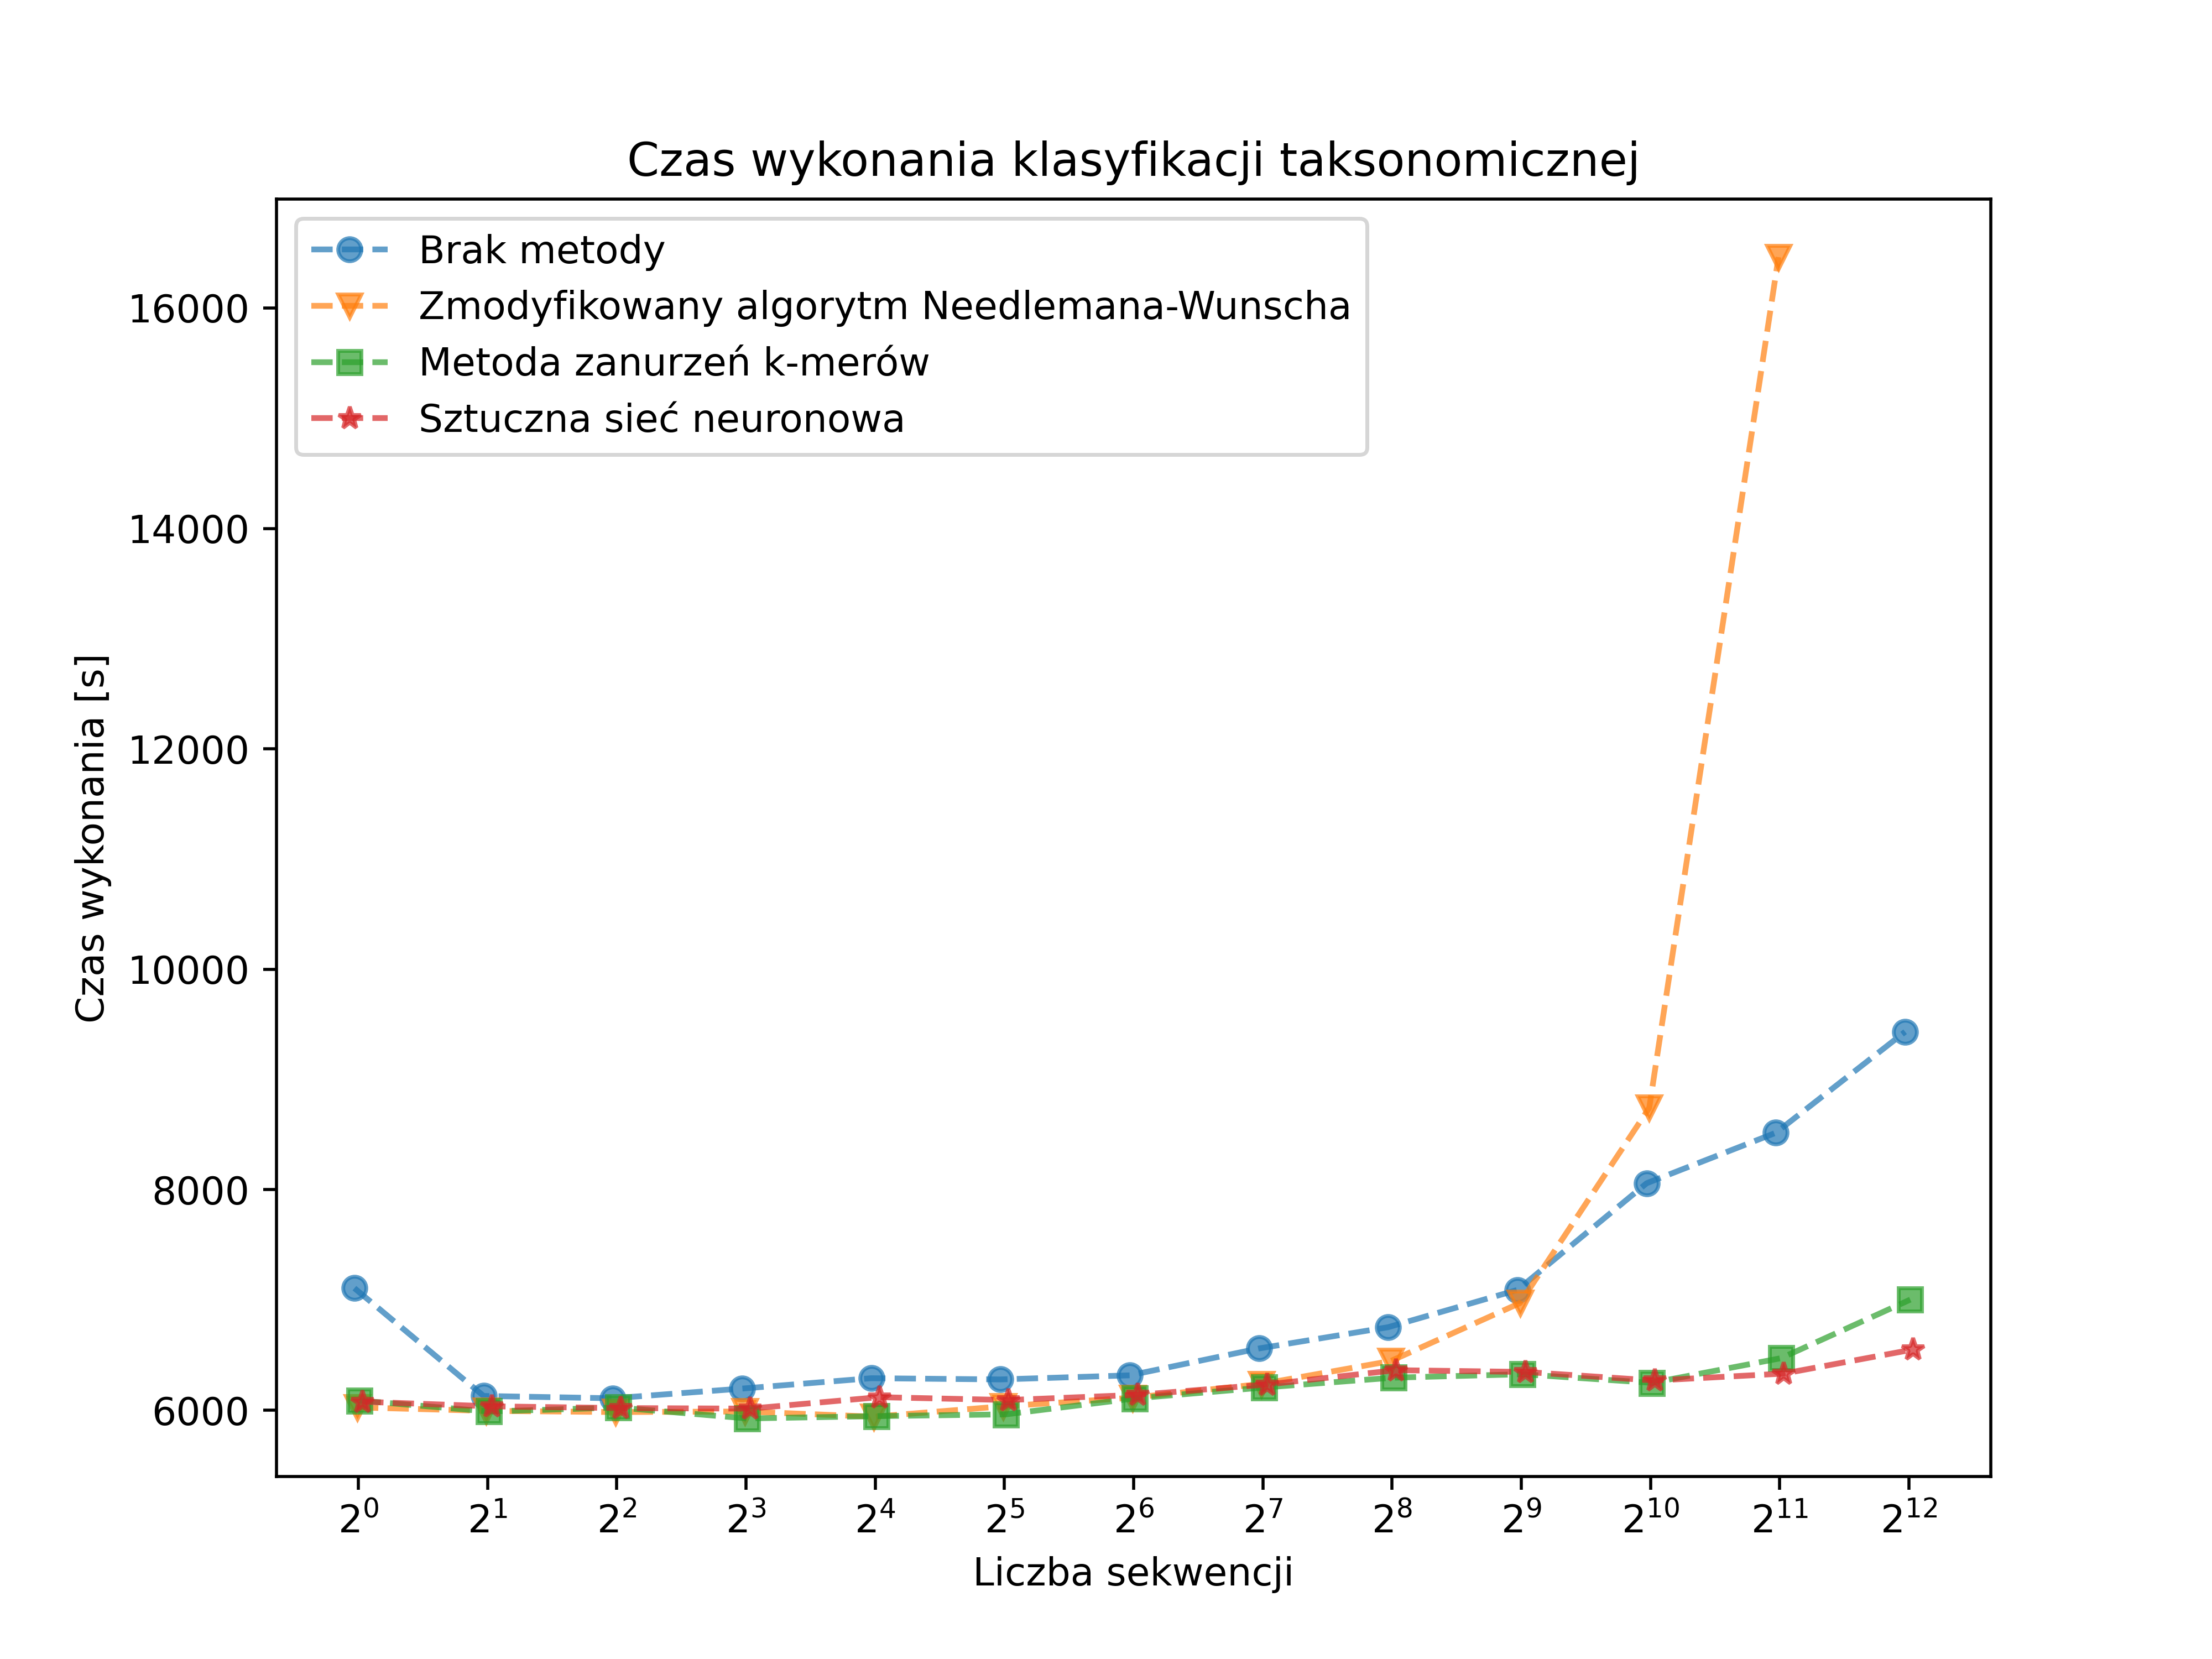
\includegraphics[width=\textwidth]{tex/pictures/exp/experiment_duration.png}
                    \end{center}
                    \caption{
                        Czas wykonania klasyfikacji taksonomicznej.
                    }\label{Picture:Experiment:Duration}
                \end{figure}

                \begin{table}\centering
                    \caption{Czas trwania eksperymentów.}\label{Table:Experiment:Duration}
                    \begin{tabularx}{\textwidth}{|c||R|R|R|R|}
                        \hline
                        \multirow{2}{*}{\textbf{Liczba sekwencji}} & \multicolumn{4}{|c|}{\textbf{Czas trwania eksperymentu}} \\ \cline{2-5}
                                        & \textbf{BZ} & \textbf{NW} & \textbf{$k$-mer} & \textbf{SSN} \\ \hline \hline
                                        1 & 7107 & \textbf{6025} & 6087 & 6077\\ \hline
                                        2 & 6129 & 5994 & \textbf{5988} & 6035\\ \hline
                                        4 & 6108 & \textbf{5983} & 6024 & 6019\\ \hline
                                        8 & 6196 & 5988 & \textbf{5925} & 6014\\ \hline
                                        16 & 6290 & \textbf{5941} & 5946 & 6118\\ \hline
                                        32 & 6279 & 6035 & \textbf{5962} & 6092\\ \hline
                                        64 & 6316 & 6113 & \textbf{6107} & 6139\\ \hline
                                        128 & 6560 & 6238 & \textbf{6206} & 6233\\ \hline
                                        256 & 6753 & 6446 & \textbf{6295} & 6363\\ \hline
                                        512 & 7091 & 6972 & \textbf{6326} & 6347\\ \hline
                                        1024 & 8059 & 8743 & \textbf{6248} & 6269\\ \hline
                                        2048 & 8517 & 16461 & 6472 & \textbf{6332}\\ \hline
                                        4096 & 9433 & \textbf{-1} & 7003 & 6550\\ \hline

                    \end{tabularx}
                \end{table}

                \begin{table}\centering
                    \caption{Wykorzystanie procesora oraz pamięci.}\label{Table:Experiment:Resources}
                    \begin{tabularx}{\textwidth}{|c||R|R|R|R||R|R|R|R|}
                        \hline
                        \multirow{2}{*}{\textbf{Liczba sekwencji}} & \multicolumn{4}{|c||}{\textbf{Wykorzystanie procesora [proc.]}} & \multicolumn{4}{|c|}{\textbf{Wykorzystanie pamięci [MB]}} \\ \cline{2-9}
                                        & \textbf{BZ} & \textbf{NW} & \textbf{$k$-mer} & \textbf{SSN} & \textbf{BZ} & \textbf{NW} & \textbf{$k$-mer} & \textbf{SSN} \\ \hline \hline
                                        1 & \textbf{14} & \textbf{14} & \textbf{14} & \textbf{14} & 37954 & 37451 & 39191 & \textbf{41120}\\ \hline
                                        2 & \textbf{15} & 14 & 14 & 14 & 37584 & 37493 & 38081 & \textbf{40567}\\ \hline
                                        4 & \textbf{16} & 14 & 14 & 14 & 37632 & 37510 & 38150 & \textbf{40701}\\ \hline
                                        8 & \textbf{18} & 14 & 15 & 13 & 37590 & 37545 & 38119 & \textbf{40685}\\ \hline
                                        16 & \textbf{22} & 15 & 16 & 17 & 37596 & 37509 & 38133 & \textbf{40781}\\ \hline
                                        32 & \textbf{21} & 15 & 16 & 15 & 37846 & 37589 & 38115 & \textbf{40766}\\ \hline
                                        64 & \textbf{21} & 17 & 17 & 17 & 37798 & 37604 & 37963 & \textbf{40706}\\ \hline
                                        128 & \textbf{26} & 21 & 20 & 19 & 37476 & 37638 & 37973 & \textbf{40396}\\ \hline
                                        256 & \textbf{32} & 25 & 22 & 20 & 37539 & 37667 & 37957 & \textbf{40385}\\ \hline
                                        512 & \textbf{38} & 33 & 25 & 23 & 37465 & 37590 & 37929 & \textbf{40414}\\ \hline
                                        1024 & \textbf{53} & 44 & 21 & 19 & 37462 & 37591 & 37876 & \textbf{40490}\\ \hline
                                        2048 & 61 & \textbf{70} & 24 & 22 & 37424 & 37607 & \textbf{37907} & 33674\\ \hline
                                        4096 & 68 & \textbf{96} & 29 & 24 & 37463 & 37504 & \textbf{37900} & 17106\\ \hline
                    \end{tabularx}
                \end{table}

            \paragraph{Wnioski}
                Metoda z wykorzystaniem zmodyfikowanego algorytmu Needlemana-Wunscha zgodnie z oczekiwaniami cechowała się najszybszym wzrostem czasu wykonania klasyfikacji taksonomicznej. Gwałtowny wzrost spowodowany jest porównywanie sekwencji każda z każdą przez budowę macierzy podobieństwa. Pomimo redukcji ilości sekwencji, które poddawane są klasyfikacji, czas wykonania tą metodą przekroczył klasyfikację taksonomiczną wszystkich sekwencji bez wykorzystania potoku przetwarzania.

                Metody z wykorzystaniem zanurzeń $k$-merów oraz sztucznej sieci neuronowej cechowały się porównywalnymi czasami wykonania z lekką przewagą dla pierwszej metody. Obie metody działały szybciej od klasyfikacji taksonomicznej bez wykorzystania potoku przetwarzania. Metody do porównywania wykorzystują reprezentacje sekwencji, co spowodowało powolniejszy wzrost czasu wykonania klasyfikacji taksonomicznej. W przypadku metody ze sztuczną siecią neuronową krótszy czas wykonania dla $4096$ sekwencji może być spowodowany obliczaniem zanurzeń dla wszystkich sekwencji jednocześnie za pomocą karty graficznej.

                W przypadku wykorzystania zasobów zauważono wzrost średniego wykorzystania procesora przez klasyfikację taksonomiczną z wykorzystaniem zaimplementowanych metod w miarę wzrostu czasu wykonania klasyfikacji, co jest związane ze znacznym nakładem obliczeniowym podczas tworzenia macierzy niepodobieństwa, której złożoność tworzenia rośnie kwadratowo wraz z liczbą sekwencji.

                Zauważalne również jest większe wykorzystanie pamięci RAM przez metodę ze sztuczną siecią neuronową, co spowodowane jest koniecznością wczytania modelu sztucznej sieci neuronowej do pamięci.

        \subsubsection{Eksperyment 2: Jakość klasyfikacji taksonomicznej}

            \paragraph{Cel}
                Celem drugiego eksperymentu było zbadanie jakości klasyfikacji taksonomicznej z wykorzystaniem zaimplementowanych metod względem klasyfikacji taksonomicznej wszystkich sekwencji. Zbadano również tworzone grupy przez zaimplementowane metody.

            \paragraph{Założenia}

                \begin{enumerate}
                    \item {
                        Proces tworzenia grup przebiega deterministycznie.
                    }
                    \item {
                        Program \texttt{BLASTn} działa deterministycznie, zwracając dla danej sekwencji i zadanych parametrów zawsze te same wyniki.
                    }
                    \item {
                        W przypadku braku możliwości obliczenia jakości dla danego przebiegu klasyfikacji taksonomicznej za wartość jakości przyjęto $0$, wartość ta nie jest brana pod uwagę w przypadku obliczania średniej jakości ważonej.
                    }
                \end{enumerate}

            \paragraph{Wyniki}
                Obliczono jakość klasyfikacji za pomocą miary wyrażonej wzorem~\ref{Equation:Quality} dla zaimplementowanych metod względem pełnej klasyfikacji taksonomicznej. Na rysunku~\ref{Picture:Experiment:Quality} przedstawiono wykres jakości klasyfikacji w zależności od ilości sekwencji wejściowych, szczegółowe wyniki jakości umieszczono w tabeli~\ref{Table:Experiment:Quality}. Średnia ważona jakość obliczona za pomocą wzoru~\ref{Equation:WeightedAverageQuality} dla metody ze zmodyfikowanym algorytmem Needlemana-Wunscha wyniosła $0,899$, dla metody z zanurzeniami $k$-merów wyniosła $0,921$, natomiast dla metody z wykorzystaniem sztucznej sieci neuronowej $0,944$. Na rysunku~\ref{Picture:Experiment:RelativeQualityNMI} przedstawiono wykres jakości względnej grup obliczony za pomocą wzoru~\ref{Equation:NMI}, natomiast na rysunku~\ref{Picture:Experiment:RelativeQualitySensitivity} przedstawiono wykres czułości obliczonej za pomocą wzoru~\ref{Equation:Sensitivity} reprezentantów grup. Szczegółowe wyniki znajdują się odpowiednio w tabeli~\ref{Table:Experiment:RelativeQualityNMI} oraz tabeli~\ref{Table:Experiment:RelativeQualitySensitivity}.

                \begin{figure}[!htb]
                    \begin{center}
                        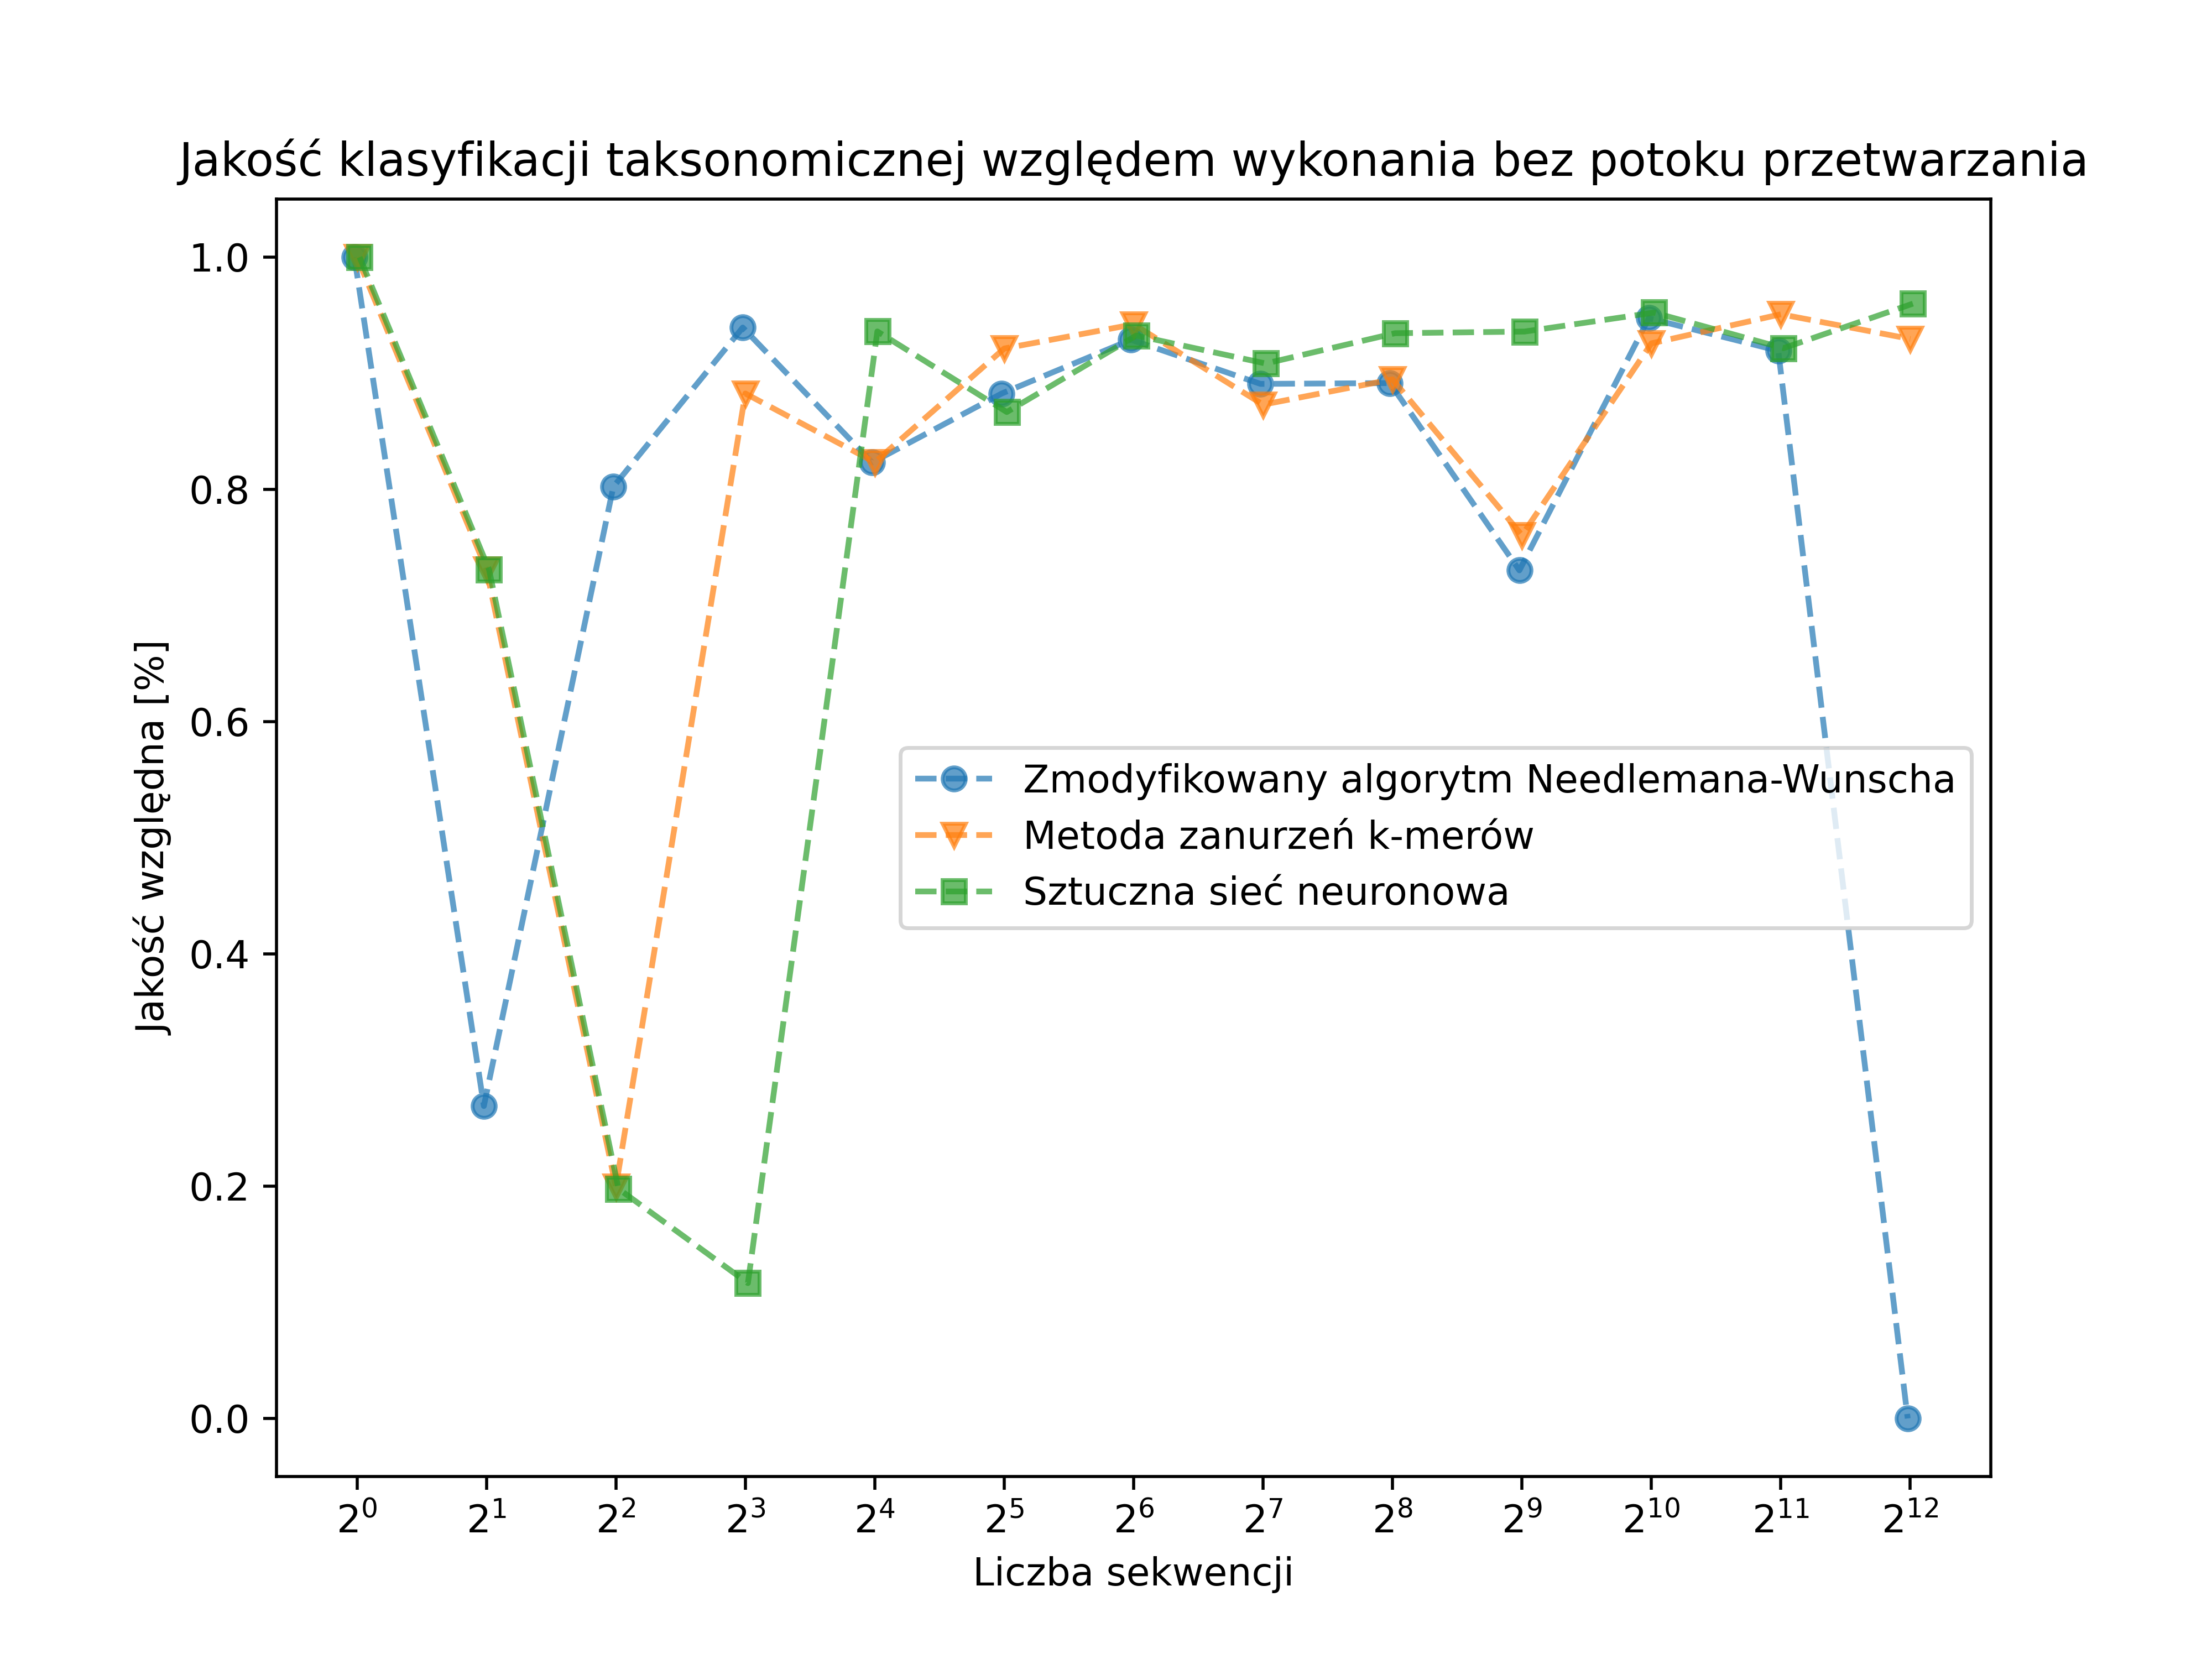
\includegraphics[width=\textwidth]{tex/pictures/exp/experiment_quality.png}
                    \end{center}
                    \caption{
                        Jakość klasyfikacji taksonomicznej.
                    }\label{Picture:Experiment:Quality}
                \end{figure}

                \begin{table}\centering
                    \caption{Jakość klasyfikacji taksonomicznej.}\label{Table:Experiment:Quality}

                    \begin{tabularx}{\textwidth}{|c|R|R|R|}
                        \hline
                        \multirow{2}{*}{\textbf{Liczba sekwencji}} & \multicolumn{3}{|c|}{\textbf{Metoda}} \\ \cline{2-4}
                        & \textbf{NW} & \textbf{$k$-mer} & \textbf{SSN} \\ \hline \hline
                        1 & \textbf{1,0} & \textbf{1,0} & \textbf{1,0}\\ \hline
                        2 & 0,27 & \textbf{0,73} & \textbf{0,73}\\ \hline
                        4 & \textbf{0,8} & 0,2 & 0,2\\ \hline
                        8 & \textbf{0,94} & 0,88 & 0,12\\ \hline
                        16 & 0,82 & 0,82 & \textbf{0,94}\\ \hline
                        32 & 0,88 & \textbf{0,92} & 0,87\\ \hline
                        64 & 0,93 & \textbf{0,94} & 0,93\\ \hline
                        128 & 0,89 & 0,87 & \textbf{0,91}\\ \hline
                        256 & 0,89 & 0,89 & \textbf{0,93}\\ \hline
                        512 & 0,73 & 0,76 & \textbf{0,94}\\ \hline
                        1024 & \textbf{0,95} & 0,93 & \textbf{0,95}\\ \hline
                        2048 & 0,92 & \textbf{0,95} & 0,92\\ \hline
                        4096 & 0,0 & 0,93 & \textbf{0,96}\\ \hline
                    \end{tabularx}
                \end{table}

                \begin{figure}[!htb]
                    \begin{center}
                        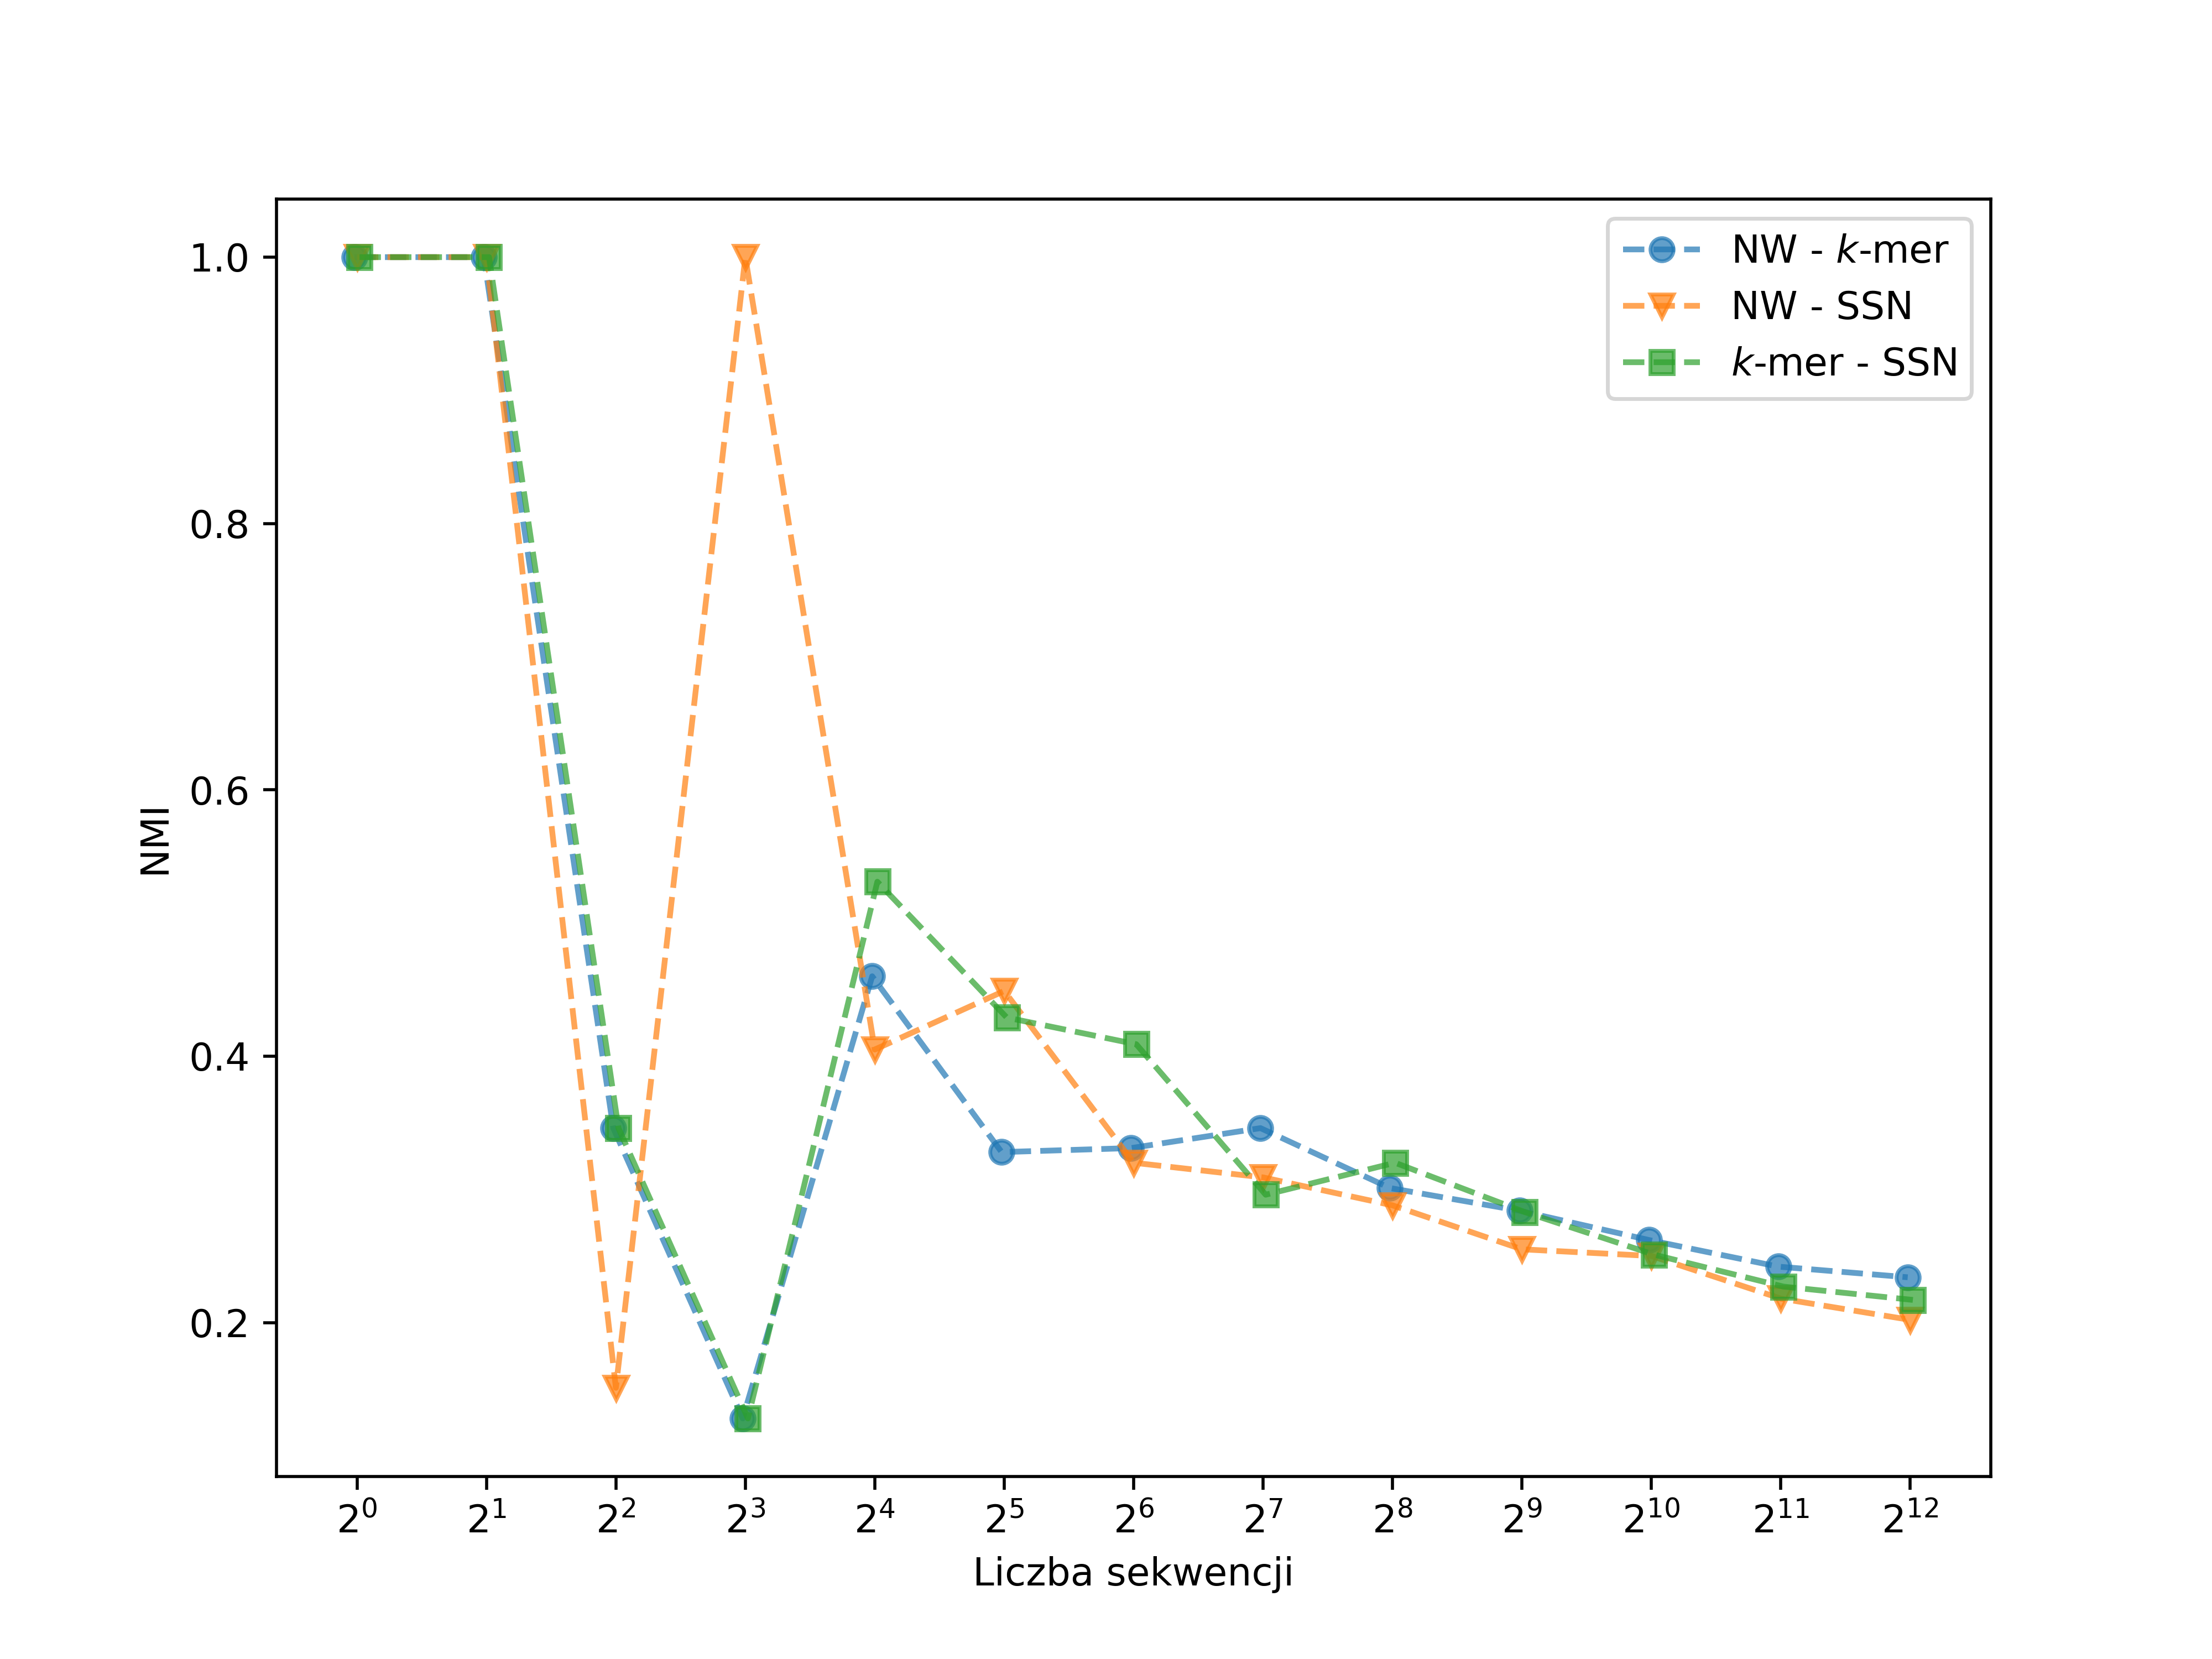
\includegraphics[width=\textwidth]{tex/pictures/exp/experiment_relative_quality_nmi.png}
                    \end{center}
                    \caption{
                       Jakość względna grup wykorzystywanych w klasyfikacji taksonomicznej.
                    }\label{Picture:Experiment:RelativeQualityNMI}
                \end{figure}

                \begin{figure}[!htb]
                    \begin{center}
                        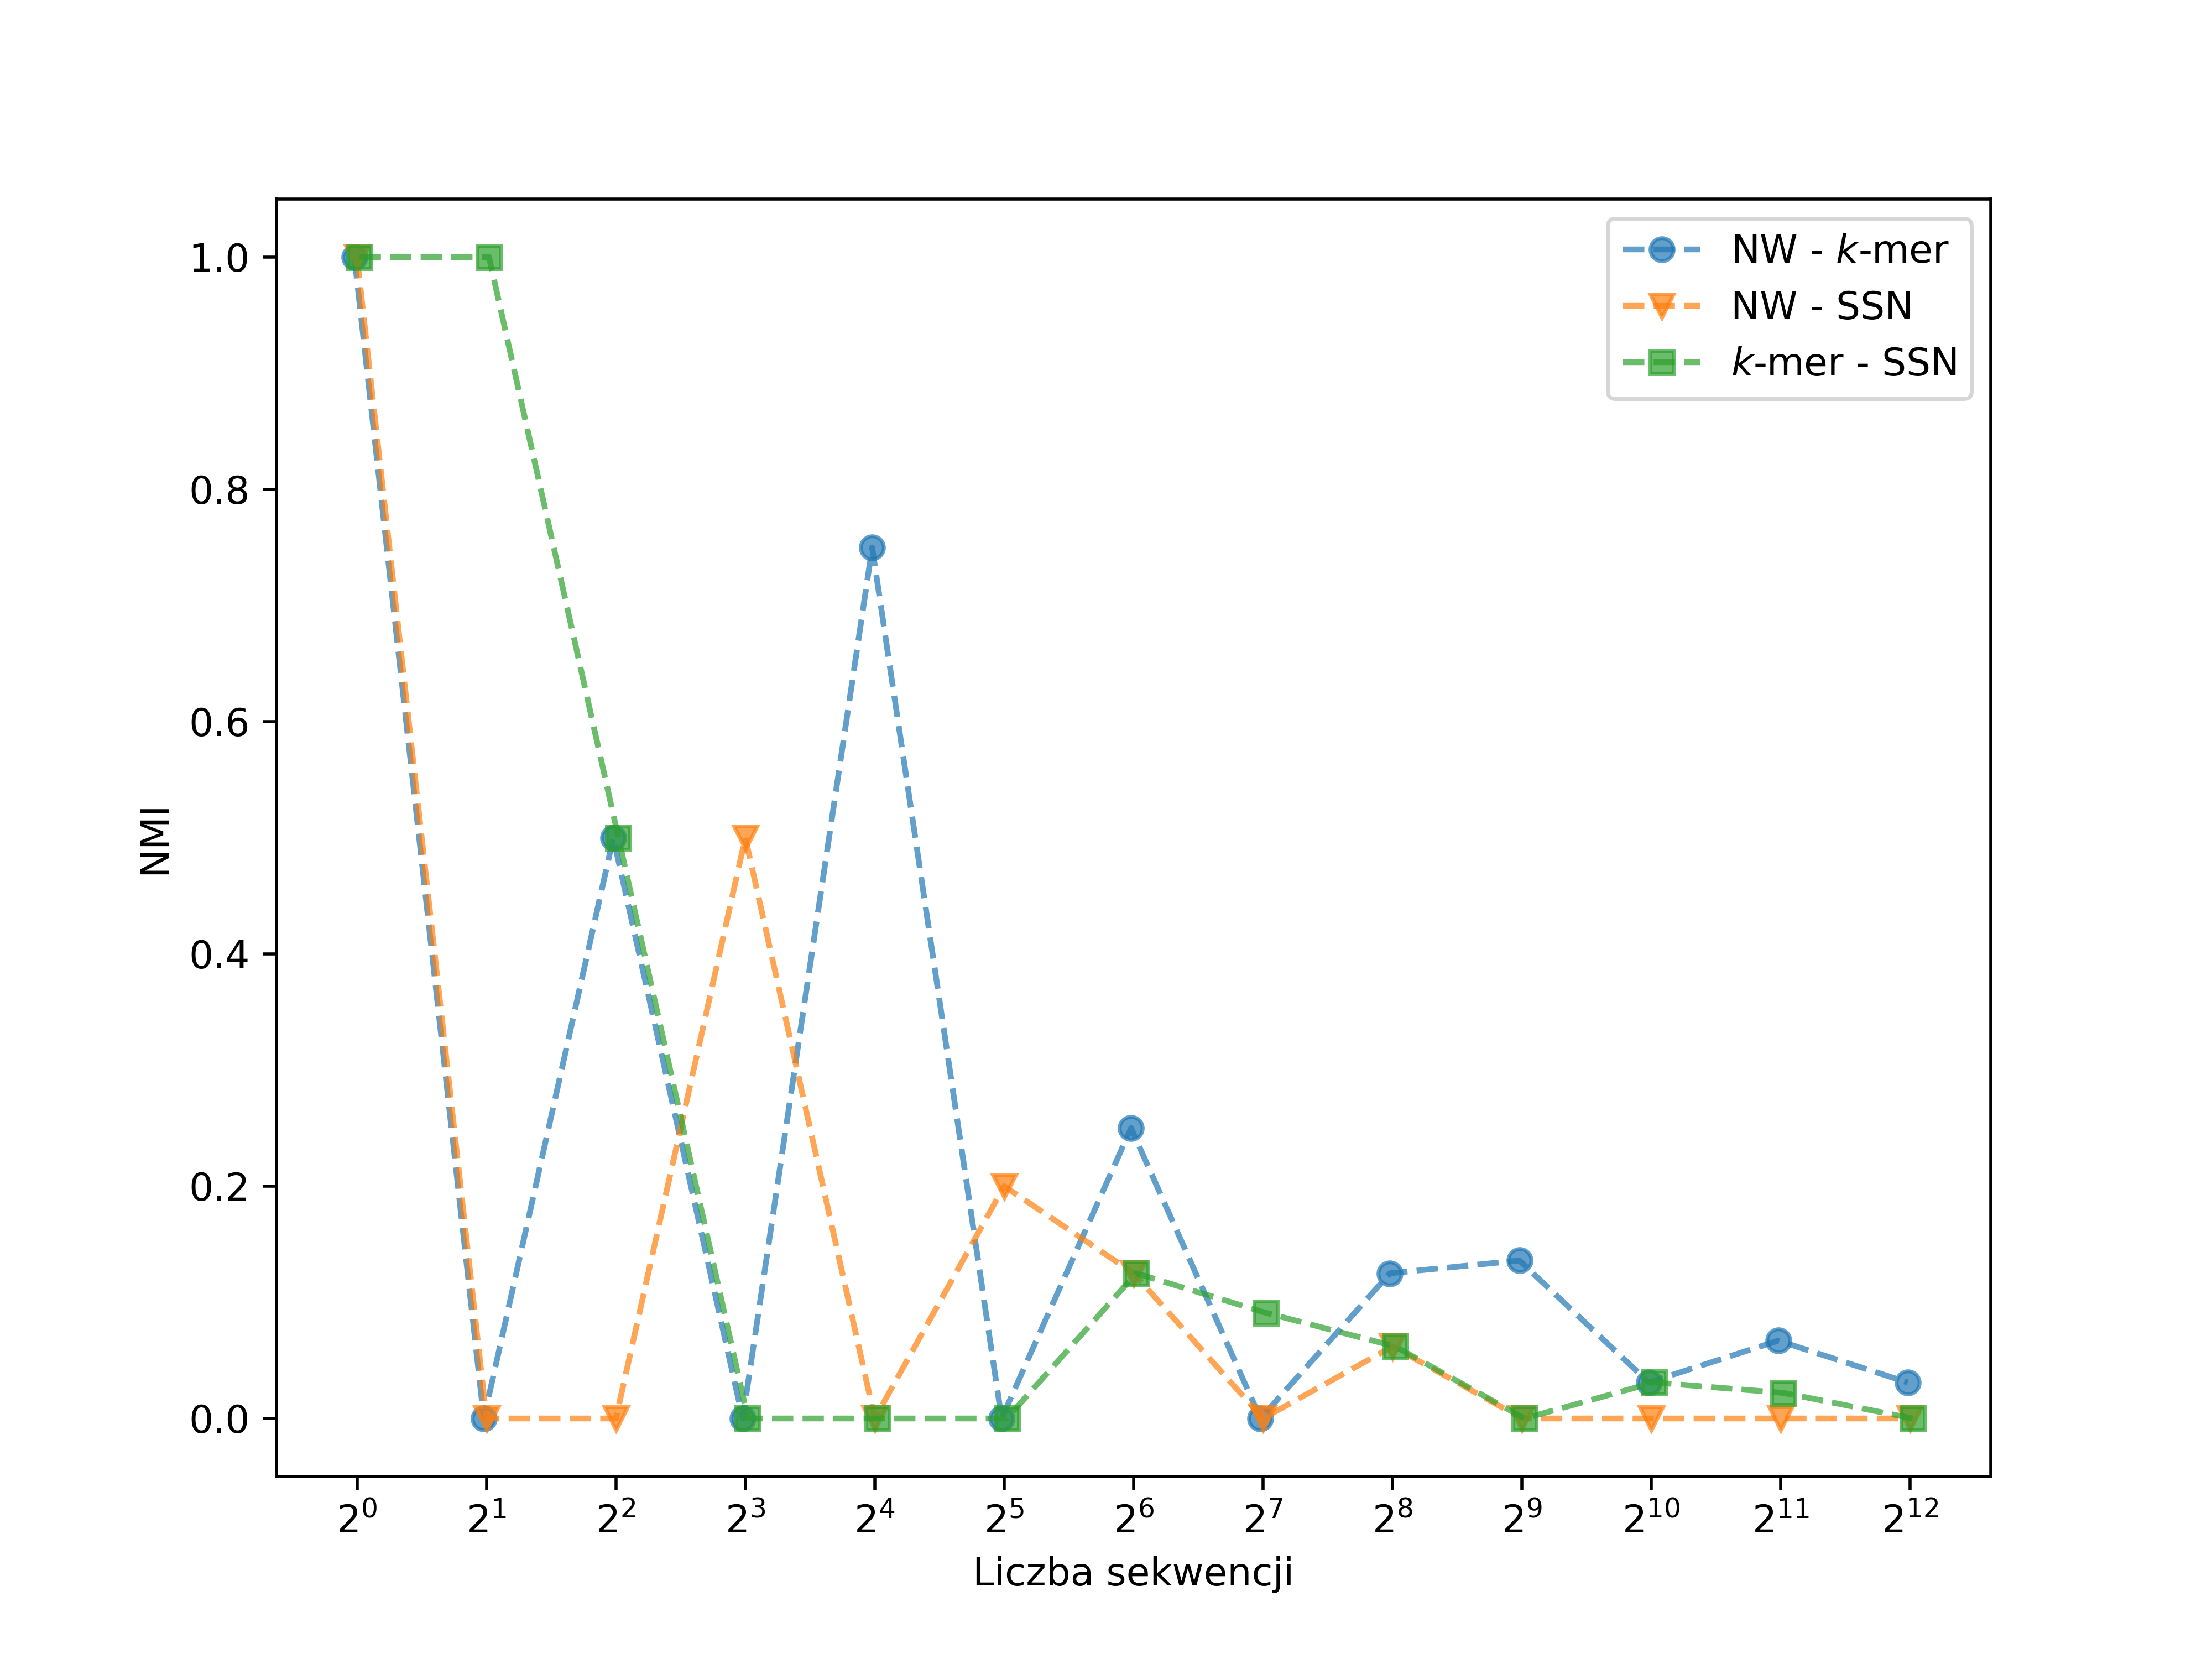
\includegraphics[width=\textwidth]{tex/pictures/exp/experiment_relative_quality_sensitivity.png}
                    \end{center}
                    \caption{
                       Czułość między reprezentantami grup wykorzystanych w klasyfikacji taksonomicznej.
                    }\label{Picture:Experiment:RelativeQualitySensitivity}
                \end{figure}

                \begin{table}\centering
                    \caption{Jakość względna grup wykorzystywanych w klasyfikacji taksonomicznej.}\label{Table:Experiment:RelativeQualityNMI}

                    \begin{tabularx}{\textwidth}{|c|R|R||R|}
                        \hline
                        \multirow{2}{*}{\textbf{Liczba sekwencji}} & \multicolumn{3}{|c|}{\textbf{Metoda}} \\ \cline{2-4}
                        & \textbf{NW - $k$-mer} & \textbf{NW - SSN} & \textbf{$k$-mer - SSN} \\ \hline \hline
                        1 & 1 & 1 & 1\\ \hline
                        2 & 1 & 1 & 1\\ \hline
                        4 & 0,346 & 0,151 & 0,346\\ \hline
                        8 & 0,128 & 1,0 & 0,128\\ \hline
                        16 & 0,46 & 0,405 & 0,531\\ \hline
                        32 & 0,328 & 0,449 & 0,429\\ \hline
                        64 & 0,331 & 0,32 & 0,409\\ \hline
                        128 & 0,346 & 0,309 & 0,296\\ \hline
                        256 & 0,301 & 0,288 & 0,32\\ \hline
                        512 & 0,284 & 0,255 & 0,283\\ \hline
                        1024 & 0,262 & 0,25 & 0,251\\ \hline
                        2048 & 0,242 & 0,218 & 0,227\\ \hline
                        4096 & 0,234 & 0,202 & 0,217\\ \hline
                    \end{tabularx}
                \end{table}

                \begin{table}\centering
                    \caption{Czułość między reprezentantami grup wykorzystanych w klasyfikacji taksonomicznej.}\label{Table:Experiment:RelativeQualitySensitivity}

                    \begin{tabularx}{\textwidth}{|c|R|R||R|}
                        \hline
                        \multirow{2}{*}{\textbf{Liczba sekwencji}} & \multicolumn{3}{|c|}{\textbf{Metoda}} \\ \cline{2-4}
                        & \textbf{NW - $k$-mer} & \textbf{NW - SSN} & \textbf{$k$-mer - SSN} \\ \hline \hline
                        1 & 1,0 & 1,0 & 1,0\\ \hline
                        2 & 0,0 & 0,0 & 1,0\\ \hline
                        4 & 0,5 & 0,0 & 0,5\\ \hline
                        8 & 0,0 & 0,5 & 0,0\\ \hline
                        16 & 0,75 & 0,0 & 0,0\\ \hline
                        32 & 0,0 & 0,2 & 0,0\\ \hline
                        64 & 0,25 & 0,125 & 0,125\\ \hline
                        128 & 0,0 & 0,0 & 0,091\\ \hline
                        256 & 0,125 & 0,062 & 0,062\\ \hline
                        512 & 0,136 & 0,0 & 0,0\\ \hline
                        1024 & 0,031 & 0,0 & 0,031\\ \hline
                        2048 & 0,067 & 0,0 & 0,022\\ \hline
                        4096 & 0,031 & 0,0 & 0,0\\ \hline
                    \end{tabularx}
                \end{table}

            \paragraph{Wnioski}
                Wszystkie zaimplementowane metody osiągnęły bardzo dobre wyniki jakości klasyfikacji, przekraczając $0,7$, w przypadkach, gdy liczba grup była znacznie większa od ilości sekwencji wejściowych. Średnia jakość ważona dla wszystkich metod również osiągnęła wysoką wartość.
                Metoda z wykorzystaniem sztucznej sieci neuronowej osiągnęła najlepszy wynik średniej jakości ważonej, wyprzedzając nieznacznie metodę z zanurzeniami $k$-merów oraz metodę ze zmodyfikowanym algorytmem Needlamana-Wunscha. Wbrew oczekiwaniom, metoda Needlemana-Wunscha osiągnęła najniższy wynik spośród zaimplementowanych metod.
                Metoda z wykorzystaniem sztucznej sieci neuronowej zawdzięcza swój wynik uwzględnieniu pełnej struktury sekwencji przez model, co pozwoliło na lepsze określenie niepodobieństwa między sekwencjami.
                Powolny spadek znormalizowanej informacji wzajemnej wraz ze wzrostem ilości sekwencji wejściowych świadczy o tworzeniu coraz mniej podobnych grup przez algorytm grupowania w wyniku zastosowania różnych metod do wyznaczania niepodobieństwa. Najbardziej podobne zbiory grup były tworzone między metodą ze zmodyfikowanym algorytmem Needlemana-Wunscha a metodą z zanurzeniami $k$-merów.

        \subsubsection{Analiza wyników}

            Wyniki eksperymentów częściowo potwierdziły oczekiwania postawione na początku badań. Wszystkie metody osiągnęły zadowalającą jakość klasyfikacji taksonomicznej. Szczególnie dobrze wypadła metoda wykorzystująca sztuczną sieć neuronową, która osiągnęła najlepszą średnią ważoną jakość klasyfikacji jednocześnie zachowując czas wykonania porównywalny z metodą opartą na zanurzeniach $k$-merów. Metoda Needlemana-Wunscha nie spełniła oczekiwań, będąc najwolniejszą metodą i osiągając wbrew oczekiwaniom jednocześnie najgorsze wyniki jakości klasyfikacji. Niska jakość klasyfikacji taksonomicznej przy małej liczbie sekwencji wejściowych może wynikać z nieodpowiedniego wyboru reprezentantów grup, co jest spowodowane zbyt małą liczbą dostępnych sekwencji. Zaimplementowane metody powinny być więc stosowane jedynie w przypadkach, gdy liczba sekwencji wejściowych przekracza pewien próg i ich wykorzystanie realnie skraca czas procesu klasyfikacji taksonomicznej. Dla badanych danych warunek ten jest osiągnięty dla $128$ sekwencji, gdzie jakość klasyfikacji taksonomicznej wynosiła nie mniej niż $0,87$, a wykorzystanie dowolnej metody grupowania skraca czas o co najmniej 5 minut, co stanowi przyśpieszenie o $5\%$ względem klasyfikacji taksonomicznej wszystkich sekwencji.


\cleardoublepage
\section{Podsumowanie}

    % ===== ===== ===== =====
    % GŁÓWNE CELE PRACY
    % ===== ===== ===== =====
    \subsection{Główne cele pracy}
        \todo{
            \begin{enumerate}
                \item {krótkie przepomnienie celu pracy oraz eksperymentów,}
                \item {podsumowanie problemów, które zostały rozwiązane}
            \end{enumerate}
        }

    % ===== ===== ===== =====
    % WYNIKI I OSIĄGNIĘCIA
    % ===== ===== ===== =====
    \subsection{Wyniki i osiągnięcia}
        \todo{
            \begin{enumerate}
                \item {najważniejsze cechy wytworzonego rozwiązania,}
                \item {wnioski z eksperymentów}
            \end{enumerate}
        }

    % ===== ===== ===== =====
    % OGRANICZENIA
    % ===== ===== ===== =====
    \subsection{Ograniczenia}

        \subsubsection{Ograniczona funkcjonalność narzędzi do sieci neuronowych w Rust}

            Mimo rosnącej popularności języka Rust\cite{Rust:popularity} i dynamicznego rozwoju jego ekosystemu, narzędzia do tworzenia modeli sztucznych sieci neuronowych są nadal w fazie rozwoju. Dostępne biblioteki w większości oferują interfejsy do istniejących rozwiązań w języku C++ lub w mniejszym stopniu są pisane od podstaw. Ze względu na wczesny etap rozwoju pierwszy typ tych narzędzi nie wykorzystuje w pełni możliwości języka Rust, a drugi typ nie zapewnia jeszcze pełnej optymalizacji procesu uczenia modeli sztucznych sieci neuronowych w porównaniu do bardziej dojrzałych rozwiązań dostępnych w językach C++ czy Python. Wykorzystana w pracy biblioteka \texttt{burn} wraz ze środowiskiem \texttt{wgpu} napotkała ograniczenia, które uniemożliwiły w pełni wykorzystanie potencjału dostępnej karty graficznej. Biblioteka na obecnym poziomie rozwoju zawiera jedynie implementacje podstawowych i klasycznych rozwiązań w dziedzinie sztucznych sieci neuronowych.

        \subsubsection{Złożoność procesu uczenia modelu sztucznej sieci neuronowej}

            Wykorzystanie dużego zbioru uczącego zawierającego milion przykładów w procesie uczenia znacząco spowolniło proces uczenia oraz strojenia modelu sztucznej sieci neuronowej. Ze względu na ograniczenia wykorzystanego narzędzia do tworzenia modelu wykonanie jednej epoki trwało około 1 godzinę na karcie graficznej NVIDIA RTX 2060 Super. Wybór tak dużego zbioru uczącego był podyktowany wysoką złożonością przestrzeni danych, której rozmiar w przypadku wykorzystania sekwencji DNA o długości 150 wynosi $4^{150}$, co daje w przybliżeniu $10^{90}$ różnych sekwencji DNA. W uczeniu kontrastowym wykorzystanie dużych zbiorów danych pozwala na stworzenie lepszego modelu, który uwzględnia więcej informacji o strukturze sekwencji.

        \subsubsection{Czasochłonność eksperymentów}

            Przeprowadzenie całego procesu klasyfikacji taksonomicznej sekwencji DNA z wykorzystaniem narzędzia \texttt{BLASTn} w ramach eksperymentów dla każdej metody i każdego podzbioru eksperymentalnego było procesem czasochłonnym. Łączny czas wykonania eksperymentów opisanych w pracy wyniósł około 5 dni, co spowodowało ograniczenie liczby eksperymentów do jednego przebiegu i rozmiaru podzbioru eksperymentalnego do maksymalnie $4096$ sekwencji.

        \subsubsection{Wykorzystanie jednego zbioru danych}

            W pracy wykorzystano jedynie część dostępnego zbioru danych, ograniczając się do jednej próbki ze względu na jej duży rozmiar. Wybór próbki zawierającej sekwencje DNA pochodzące z mikrobiomu skóry człowieka mógł ograniczyć przestrzeń analizowanych sekwencji, co mogło wpłynąć na wyniki eksperymentów, ponieważ w eksperymentach również wykorzystano sekwencje DNA pochodzące z tego samego mikrobiomu.

        \subsubsection{Złożoność obliczeniowa macierzy niepodobieństwa}

            Czas budowy macierzy niepodobieństwa rośnie wprost proporcjonalnie do kwadratu liczby sekwencji, które zostały użyte do jej budowy. Macierz niepodobieństwa wykorzystywana przez algorytm grupowania w pracy była budowana dla wszystkich sekwencji wejściowych. Zastosowane podejście znacznie ogranicza liczbę możliwych sekwencji wejściowych ze względu na szybki wzrost czasu potrzebnego na tworzenie macierzy niepodobieństwa.

    % ===== ===== ===== =====
    % MOŻLIWOŚCI DALSZEGO ROZWOJU
    % ===== ===== ===== =====
    \subsection{Możliwości dalszego rozwoju}

        \subsubsection{Zmiana architektury modelu sztucznej sieci neuronowej}

            Stworzony model sztucznej sieci neuronowej wymaga sekwencji o stałej długości, co ogranicza elastyczność modelu w analizie sekwencji o różnych długościach i wymaga tworzenia nowego modelu dostosowanego do dłuższych sekwencji w przypadku znacznej różnicy między długościami sekwencji wejściowych a oczekiwanych przez model. Dodatkowo sekwencje krótsze niż wymagane wymagają wydłużenia do zadanej długości przez wypełnienie wybraną zasadą. W przyszłości można rozważyć zmianę architektury modelu sztucznej sieci neuronowej, dostosowując ją do analizy sekwencji o zmiennych długościach poprzez zastosowanie sieci rekurencyjnych lub typu LSTM w pierwszych warstwach modelu.

        \subsubsection{Grupowanie sekwencji w paczkach}

            Ze względu na czasochłonność procesu budowy macierzy niepodobieństwa, na wstępnym etapie sekwencje wejściowe mogłyby zostać poddane losowemu grupowaniu w paczki. Następnie, w ramach każdej paczki, przeprowadzony zostałby proces wyboru reprezentantów, tak jak ma to miejsce w obecnym podejściu. Zastosowanie wstępnego grupowania umożliwiłoby ominięcie budowy jednej dużej macierzy niepodobieństwa, co pozwoliłoby na analizę większej liczby sekwencji.

        \subsubsection{Wykonywanie obliczeń równolegle}

            Możliwa jest optymalizacja niektórych operacji wykonywanych w potoku przetwarzania poprzez zastosowanie obliczeń równoległych. Pierwszym elementem, w którym można wykorzystać obliczenia równoległe, jest budowa macierzy niepodobieństwa. Macierz tą można podzielić na fragmenty, które będą budowane równolegle i niezależnie. Drugą zmianą jest modyfikacja potoku przetwarzania, która pozwalałaby na równoczesne wykonywanie niektórych etapów, bez konieczności oczekiwania na zakończenie obliczeń w innych częściach potoku. Przykładem takiego etapu jest wyliczanie zanurzeń, które mogłoby być wykorzystywane bezpośrednio do budowy macierzy niepodobieństwa bez oczekiwania na obliczenie wszystkich zanurzeń.

        \subsubsection{Automatyczny dobór liczby grup}

            Obecne podejście wymaga doboru liczby tworzonych grup przez algorytm grupowania. Liczba grup bezpośrednio determinuje liczbę reprezentantów, którzy będą poddani klasyfikacji taksonomicznej i ma wpływ na jakość oraz czas wykonania całego procesu. Możliwe byłoby zastosowanie lub stworzenie algorytmu, który automatycznie dobierałby liczbę tworzonych grup na podstawie macierzy niepodobieństwa oraz miar jakości tworzonych grup. Automatyczne dostosowanie liczby grup pozwoliłoby na zwiększenie jakości klasyfikacji w przypadku bardzo różnych sekwencji wejściowych bez spowalniania procesu dla zbiorów sekwencji bardzo podobnych.

        \subsubsection{Narzędzie do klasyfikacji taksonomicznej oparte o model sztucznej sieci neuronowej}

            Narzędzia do klasyfikacji taksonomicznej w większości opierają się na obliczaniu podobieństwa między sekwencjami wejściowymi a sekwencjami znajdującymi się w bazie danych sekwencji w celu znalezienia sekwencji, które są podobne. Wykorzystane w eksperymentach narzędzie \texttt{BLASTn} wykorzystuje $k$-mery do określenia podobieństwa między sekwencjami. 
            Grupowanie sekwencji, które zostało wykorzystane w pracy, wykonuje podobne operacje, do tych, które są wykonywane przez narzędzia do klasyfikacji taksonomicznej. Możliwe byłoby zatem stworzenie własnego narzędzia, które wykorzystywałoby bezpośrednio model sztucznej sieci neuronowej do określenia podobieństwa między sekwencjami i klasyfikacji taksonomicznej. Wykorzystanie sztucznych sieci neuronowych w przypadku wydajnej implementacji mogłoby pozwolić na osiągnięcie akceptowalnego czasu działania przy wyższej jakości.

    % ===== ===== ===== =====
    % WNIOSKI KOŃCOWE
    % ===== ===== ===== =====
    \subsection{Wnioski końcowe}

        \todo{
            \begin{enumerate}
                \item {podsumowanie głównych wniosków z pracy,}
                \item {podkręslenie najważniejszych osiągnięć}
            \end{enumerate}
        }

\begin{enumerate}
    \item Spis literatury [30 prac]

    \item Spis rysunków
\end{enumerate}

% ---- ---- ---- ----
% Bibliography
% ---- ---- ---- ----
\cleardoublepage % Zaczynamy od nieparzystej strony
\printbibliography
\clearpage

% ---- ---- ---- ----
% Wykaz symboli i skrótów
% ---- ---- ---- ----

% ---- ---- ---- ----
% Spis rysunków
% ---- ---- ---- ----
\pagestyle{plain}
\listoffigurestoc{}
\vspace{1cm}

% ---- ---- ---- ----
% Spis tabel
% ---- ---- ---- ----
\listoftablestoc{}

% ---- ---- ---- ----
% Spis załączników
% ---- ---- ---- ----
    % Empty

% ---- ---- ---- ----
% Załączniki
% ---- ---- ---- ----
    % Empty

\end{document}